\begingroup
\usingnamespace{nstar:grammar}
\usingnamespace{nstar:rules}



\part{The back end}\label{part:nstar}


\chapter{Introduction}\label{chap:nstar-abstract}

Assembly languages are the lowest level of humanly-possible programming there exists nowadays. They were used back in the days for very performance-critical tasks, or even just for fun, as there weren't many other programming languages available. Nowadays, with all the existing ones, most people have never used any assembly language.

Despite their apparent simplicity, and the small amount of work you need to put into creating assembly languages, those are in fact very hard to use. At that low level, there is no such thing as Java's exceptions keeping you from doing dumb things, Rust's linear types keeping you from leaking memory nor even Garbage Collectors. The nice things preventing you from having segfaults simply do not exist, and you are expected to either provide all those things yourself (creating a language runtime) or be very careful about what you are doing each time you write a single instruction (even a simple \texttt{mov} can have undesirable side-effects).

Doing dumb things is something that we must prevent directly when using the language. That way, we do not need to rely on external verification tools or debuggers, trying to know why a program segfaults at a specific point.
This is where a type system can become handy. Typed assembly languages are assembly languages augmented with simple yet powerful type system. Among the most famous typed assembly languages are TALx86~\cite{TALx86}, FunTAL~\cite{FunTAL} and DTAL~\cite{DTAL}.

TALx86 is basically NASM with a type system, targetting only the x86 architecture. DTAL is much more complicated and embeds a completely dependent type system. FunTAL is a more complex system than TALx86 (it is based on STAL~\cite{STAL}) and provides a fully-fledged type assembly language, almost entirely integrated inside a functional programming language.

\vspace{\baselineskip}

\nstar's goal is to assist users with a simple but powerful type system, yet still allowing for low-level data manipulation.
But before even being a usable programming language, \nstar\ aims at being a compiler backend (much like for example LLVM), and is used that way in the Zilch project. Differences with other compiler backends are mostly the type-system, allowing the compilation of Zilch source code into type-safe instructions.

\vspace{\baselineskip}

Because \nstar\ supports compiling to multiple architectures, using different grammars, describing \nstar\ will at first be platform-agnostic, treating common aspects between all CPU architectures, and then will be divided into multiple categories, explaining in more details some features on a per-architecture basis\footnote{Note that the target executable format (ELF, PE, \ldots) is also considered as an architecture-specific thing, but should not influence \nstar\ much.}.

\section*{Small notes on the notation used in the next chapters}\label{sec:nstar-abstract-notation}

\begin{itemize}
	\item Kind inference
	      \begin{itemize}
		      \item $\Gamma$ is the typing context, containing every bindings from names to type variables;
		      \item $\vdash^{\text{\tiny K}}$ is the kind inference judgement;
	      \end{itemize}
	\item Type inference
	      \begin{itemize}
		      \item $\Xi$ is the context containing all bound labels, composed of two other contexts: $\Xi_{c}$ and $\Xi_{d}$. $\Xi_{c}$ contains all the labels defined in \texttt{code} sections, and $\Xi_{d}$ contains all the labels defined in \texttt{data} sections;
		      \item $\chi$ is the current register-to-type mapping, and contains all known-to-be-bound registers.
		            A register which is not present in this context means that either it has never been bound, or the value in it has been forgotten at some point;
		      \item $\sigma$ is the current stack type;
		      \item $\epsilon$ is the current continuation;
		      \item $\vdash^{\text{\tiny T}}_{\text{\tiny data}}$ and $\vdash^{\text{\tiny T}}_{\text{\tiny code}}$ are the type inference judgements for expressions in their respective sections (\texttt{data} or \texttt{code}).
		            $\vdash^{\text{\tiny T}}_{\text{\tiny data}}$ uses no context, whereas $\vdash^{\text{\tiny T}}_{\text{\tiny code}}$ uses all four of the defined contexts above (namely $\Xi$, $\chi$, $\sigma$ and $\epsilon$);
		      \item $\ISequent{\Xi}{\Gamma}{\chi}{\sigma}{\epsilon}{instr}{\chi^\prime}{\sigma^\prime}{\epsilon^\prime}$ denotes that the type inference of the instruction $instr$ in the current typing contexts $\Xi;\Gamma;\chi;\sigma;\epsilon$ yields a new typing context $\chi^\prime;\sigma^\prime;\epsilon^\prime$ (where $\Gamma$ and $\Xi$ cannot be altered);
		      \item $t_1 \sim t_2$ (and its counterpart $t_1 \nsim t_2$) respectively mean that $t_1$ and $t_2$ can be unified (or not);
	      \end{itemize}
	\item Grammar
	      \begin{figure}[H]
		      \centering
		      \scalebox{.5}{
			      \includegraphics{grammar-template}
		      }
	      \end{figure}
	      \begin{itemize}
		      \item Normal rectangles describe other grammar rules (whose name is given in the shape);
		      \item Rounded rectangles describe terminal nodes, that is invariant string pieces;
		      \item The name of the grammar rule is given in the top-left corner of the diagram
		            For a rule to match, it must be possible to go from one end to the other while staying on the black rails;
	      \end{itemize}
\end{itemize}

\chapter{Non platform-specific features}\label{chap:nstar-common}

\section{Types}\label{sec:nstar-common-ts}

One of the differences between classical assembly languages and \nstar\ is its type system.
Compared to other higher level programming languages like Java, C++, etc, \nstar\ has a very simple yet powerful and expressive enough type system.

In programming, types are used mostly to prove at compile-time that a given program should behave well if it type-checks. While this works for more elaborated programming languages like Haskell, Idris, etc, most type systems aren't expressive enough to absolutely guarantee that everything will work at run-time (in fact, there is no possible way of doing this, because for example a memory allocation may fail, and this cannot be checked at compile-time). However, we can try to guarantee as much as possible.

\nstar\ doesn't try to solve this issue, because it would be really hard to target a dependently typed assembly language from a non-dependently typed programming language. But where all used assembly languages do not even consider types (only numbers, in fact), \nstar\ embeds a powerful type system used to remove the possibility of bugs (like incorrect structure addresses passed as a parameter function, or incoherent types in some instructions).

\subsection{Kinds}\label{subsec:nstar-common-ts-kinds}

Kinds (also known as types of types) mainly serve the purpose of indicating type sizes.
There are three type of kinds in \nstar:
\begin{itemize}
	\item Stack kind, denotating stack-like types, which can be safely offsetted
	\item Kinds whose size is abstracted away, useful to ask for any sized type
	\item Kinds whose size is already known
	\item Continuation kinds, for types that can be used as continuations
\end{itemize}
The grammar is given in Figure~\ref{fig:nstar-common-ts-kinds-syntax}.

\begin{figure}[htb]
	\centering
	\framebox[\textwidth][c]{
		\scalebox{.5}{
			\includegraphics{nstar/types/kinds-syntax}
		}
	}
	\caption{Grammar for kinds.}
	\label{fig:nstar-common-ts-kinds-syntax}
\end{figure}

\subsection{Integer types}\label{subsec:nstar-common-ts-integer}

Numbers are the building block of any assembly language. Most of data manipulated is manipulated as numbers, e.g.\ addresses, characters, strings, enumerations, etc.
This is not the case in \nstar, where ``integer''  only really means ``number''.
The syntax for the types of integers is given in Figure~\ref{fig:nstar-common-ts-integer-syntax}.

\begin{figure}[htb]
	\centering
	\framebox[\textwidth][c]{
		\scalebox{.5}{
			\includegraphics{nstar/types/integers-syntax}
		}
	}
	\caption{Grammar for integer types.}
	\label{fig:nstar-common-ts-integer-syntax}
\end{figure}

Integers have two varying parameters: their sign and sizes.
According to the sign (i.e.\ signed or unsigned), some operations may not perform the same (for example \texttt{mul} does not behave the same).
The size is nothing more than the number of bits occupied by the integer (in \nstar, those are restricted to some powers of 2 between $8$ and $64$ included).
Most operations should perform the same no matter the integer size, however it is recommended to search in the target architecture manual for further reference.

Kinds of integers are written under the form of inference rules in Figure~\ref{fig:nstar-common-ts-integer-kindrules}.

\begin{figure}[htb]
	\centering

	\framebox[\textwidth][c]{\parbox{\textwidth}{
			\centering
			\begin{prooftree}
				\infer0{\KindSequent{\Gamma}{\Tunsigned{64}}{\T8}}
			\end{prooftree}
			\hspace{3em}
			\begin{prooftree}
				\infer0{\KindSequent{\Gamma}{\Tsigned{64}}{\T8}}
			\end{prooftree}
			\hspace{3em}
			\begin{prooftree}
				\infer0{\KindSequent{\Gamma}{\Tunsigned{32}}{\T4}}
			\end{prooftree}
			\hspace{3em}
			\begin{prooftree}
				\infer0{\KindSequent{\Gamma}{\Tsigned{32}}{\T4}}
			\end{prooftree}
			\\\vspace{\baselineskip}
			\begin{prooftree}
				\infer0{\KindSequent{\Gamma}{\Tunsigned{16}}{\T2}}
			\end{prooftree}
			\hspace{3em}
			\begin{prooftree}
				\infer0{\KindSequent{\Gamma}{\Tsigned{16}}{\T2}}
			\end{prooftree}
			\hspace{3em}
			\begin{prooftree}
				\infer0{\KindSequent{\Gamma}{\Tunsigned{8}}{\T1}}
			\end{prooftree}
			\hspace{3em}
			\begin{prooftree}
				\infer0{\KindSequent{\Gamma}{\Tsigned{8}}{\T1}}
			\end{prooftree}
		}}

	\caption{Kind inference rules for integers.}
	\label{fig:nstar-common-ts-integer-kindrules}
\end{figure}

\subsection{Other atomic types}\label{subsec:nstar-common-ts-otheratomic}

There are two other atomic types that we did not talk about, but refered to in the introduction of the type system: characters and pointers. Their respective syntax is given in Figure~\ref{fig:nstar-common-ts-atomic-syntax}.

\begin{figure}[htb]
	\centering
	\framebox[\textwidth][c]{\parbox{\textwidth}{
			\centering
			\scalebox{.5}{
				\includegraphics{nstar/types/ptr-syntax}
			} \\
			\scalebox{.5}{
				\includegraphics{nstar/types/char-syntax}
			}
		}}
	\caption{Grammar for character and pointer types}
	\label{fig:nstar-common-ts-atomic-syntax}
\end{figure}

In all assembly languages, characters are merely syntactic sugar for their ASCII code. This is how their are put in the machine code anyway, so it is not a huge problem (it might even not be at all).

Pointers, on the other hand, are unabstracted memory addresses.
In \nstar, there are two types of pointers: data pointers and stack pointers.
Stack pointers are covered in Subsection~\ref{subsec:nstar-common-ts-stack}~``\nameref{subsec:nstar-common-ts-stack}''.
Data pointers simply represent an address where we know (or not, see the Subsection~\ref{subsec:nstar-common-unsafe-derefliteraladdr}~``\nameref{subsec:nstar-common-unsafe-derefliteraladdr}'') that there is a value of the given pointed type.

Kind inference is given in Figure~\ref{fig:nstar-common-ts-atomic-kindrules}.

They support two common operations: offsetting (see the Subsection~\ref{subsec:nstar-common-unsafe-ptroffset}~``\nameref{subsec:nstar-common-unsafe-ptroffset}'') and dereferencing (taking the value pointed by the pointer).
Dereferencing is considered a safe operation, unless trying to on a literal address.
There is no notion of ``null'' pointers, like \texttt{NULL} in C.
However, it is possible to use the literal \texttt{\$0} (which represents a pointer to the address $0$).

\begin{figure}[htb]
	\centering
	\framebox[\textwidth][c]{
		\begin{prooftree}
			\infer0{\KindSequent{\Gamma}{\Tchar}{\T1}}
		\end{prooftree}
		\hspace{3em}
		\begin{prooftree}
			\hypo{\KindSequent{\Gamma}{t}{\Ta}}
			\infer1[64-bits pointers]{\KindSequent{\Gamma}{\Tptr{t}}{\T8}}
		\end{prooftree}
		\hspace{3em}
		\begin{prooftree}
			\hypo{\KindSequent{\Gamma}{t}{\Ta}}
			\infer1[32-bits pointers]{\KindSequent{\Gamma}{\Tptr{t}}{\T4}}
		\end{prooftree}
	}

	\caption{Kind inference rules for other atomic types.}
	\label{fig:nstar-common-ts-atomic-kindrules}
\end{figure}

\subsection{The effectful type}\label{subsec:nstar-common-ts-effect}

The effectful type, also known as ``bang type'', is a type used to denote that some computation \textit{may} completely overwrite a value somewhere, potentially changing its type.
Its use is mainly in context types, to indicate that a function may change a register during its computation, therefore that it must be caller-saved.

Grammar and kind inference rules are given in Figure~\ref{fig:nstar-common-ts-effect-syntax} and Figure~\ref{fig:nstar-common-ts-effect-kindrules}.

\begin{figure}[htb]
	\centering

	\framebox[\textwidth][c]{\parbox{\textwidth}{
			\centering
			\scalebox{.5}{
				\includegraphics{nstar/types/bang-syntax}
			}
		}}

	\caption{Grammar for bang types.}
	\label{fig:nstar-common-ts-effect-syntax}
\end{figure}

\begin{figure}[htb]
	\centering

	\framebox[\textwidth][c]{
		\begin{prooftree}
			\infer0{\KindSequent{\Gamma}{\Tbang}{k}}
		\end{prooftree}
	}

	\caption{Type inference rules for bang types.}
	\label{fig:nstar-common-ts-effect-kindrules}
\end{figure}

\subsection{Context types}\label{subsec:nstar-common-ts-records}

Record types (or contexts) are mappings from registers to types, which also hold information about the current stack, as well as the return continuation.
They are used to indicate that a register is bound to a value of a given type at a certain point in the program.
The grammar is described in Figure~\ref{fig:nstar-common-ts-records-syntax}.

\begin{figure}[htb]
	\centering
	\framebox[\textwidth][c]{\parbox{\textwidth}{
			\centering
			\scalebox{.5}{
				\includegraphics{nstar/types/records-syntax}
			}
			\\
			\scalebox{.5}{
				\includegraphics{nstar/types/continuation-syntax}
			}
		}}
	\caption{Grammar for context and continuation types.}
	\label{fig:nstar-common-ts-records-syntax}
\end{figure}

\begin{figure}[htb]
	\centering

	\framebox[\textwidth][c]{
		\begin{prooftree}
			\hypo{\KindSequent{\Gamma}{\hat{\chi}}{}}
			\hypo{\KindSequent{\Gamma}{s}{\Ts}}
			\hypo{\KindSequent{\Gamma}{e}{\Tc}}
			\infer3{\KindSequent{\Gamma}{\Tcontext{\hat{\chi}}{s}{e}}{\Ta}}
		\end{prooftree}
	}

	\caption{Type inference rules for record types.}
	\label{fig:nstar-common-ts-records-typerules}
\end{figure}

Context types are used to represent data contexts where any mapping is some sort of a proof that some data of some type is accessible through some register.

\vspace{\baselineskip}

\textbf{Note:} In the context of label types (and more generally code addresses), a context type is augmented by a \texttt{forall} generic type variable binder.
The grammar is described in Figure~\ref{fig:nstar-common-ts-label-types-syntax}.
The type variable binder is used to abstract away some details of the type through an opaque variable specialized at the call site.

\begin{figure}[htb]
	\centering
	\framebox[\textwidth][c]{
		\scalebox{.5}{
			\includegraphics{nstar/types/label-syntax}
		}
	}
	\caption{Grammar for label context types.}
	\label{fig:nstar-common-ts-label-types-syntax}
\end{figure}

\begin{figure}[htb]
	\centering

	\framebox[\textwidth][c]{
		\begin{prooftree}
			\hypo{\KindSequent{\Gamma,\hat{v}}{\zeta}{\Ta}}
			\infer1{\KindSequent{\Gamma}{\Tforall{\hat{v}}{\zeta}}{\T8}}
		\end{prooftree}
	}

	\caption{Type inference rules for label context types.}
	\label{fig:nstar-common-ts-label-types-typerules}
\end{figure}

The example code given in Listing~\ref{lst:nstar-common-ts-records-stackmask} shows a use for type variables.
The stack is abstracted away, meaning that we can call this function from anywhere, given any stack (as long as it is \texttt{call}ed, or \texttt{jmp}ed to from a \texttt{call}ed function).
The type variable \texttt{s} is specialized at the call site.

\begin{listing}[htb]
	\centering
	\inputminted{\nstarlexer}{examples/stack-masking.nst}

	\caption{Stack masking using a type variable binder.}
	\label{lst:nstar-common-ts-records-stackmask}
\end{listing}

\subsection{Stack types}\label{subsec:nstar-common-ts-stack}

There is one stack type in \nstar: the stack constructor \texttt{::}.
Note that there is no ``empty stack'' type as would be the case with e.g.\ lists in Haskell.
The reason is that it forces the developer to abstract the stack to be able to have a ``stack tail'' (the part of the stack on the right of the stack constructor \texttt{::}) at some point.\footnote{It also serves the purpose to ensure that we cannot construct a stack from nothing, and that it should always be given to us, to e.g.\ the \texttt{main} function.}
An example is given in Listing~\ref{lst:nstar-common-ts-records-stackmask}.

The grammar for stack types is given in Figure~\ref{fig:nstar-common-ts-stack-types-syntax}.

Inference rules for kinds of stack types are written in Figure~\ref{fig:nstar-common-ts-stack-types-kindrules}

\begin{figure}[htb]
	\centering
	\framebox[\textwidth][c]{
		\scalebox{.5}{
			\includegraphics{nstar/types/stack-cons-syntax}
		}
	}
	\caption{Grammar for stack types.}
	\label{fig:nstar-common-ts-stack-types-syntax}
\end{figure}

\begin{figure}[H]
	\centering

	\framebox[\textwidth][c]{
		\begin{prooftree}
			\hypo{n\in\mathbb{N}}
			\hypo{\KindSequent{\Gamma}{t}{\T{n}}}
			\hypo{\KindSequent{\Gamma}{s}{\Ts}}
			\infer3{\KindSequent{\Gamma}{\Tstack{t}{s}}{\Ts}}
		\end{prooftree}
	}

	\caption{Kind inference rules for stack types}
	\label{fig:nstar-common-ts-stack-types-kindrules}
\end{figure}

\subsection{Structure types}\label{subsec:nstar-common-ts-structs}

Structure types are packed sets of unnamed types (compared to context types, each field does not have a name, only a type) that can be indexed from a pointer only to a full field (so if you have two \texttt{u64}s, you can only offset to $0$ and $8$, respectively for the first and second field).

Grammar is described in Figure~\ref{fig:nstar-common-ts-structs-syntax} and kind inference rules are given in Figure~\ref{fig:nstar-common-ts-structs-kindrules}.

Structures take as much space as all their fields, thus can mainly be put on the stack (unless being less than 8 bytes, which is the upper limit for register sizes in current architectures).

\begin{figure}[htb]
	\centering

	\framebox[\textwidth][c]{
		\scalebox{.5}{
			\includegraphics{nstar/types/struct-syntax}
		}
	}

	\caption{Grammar for structure types.}
	\label{fig:nstar-common-ts-structs-syntax}
\end{figure}

\begin{figure}[H]
	\centering

	\framebox[\textwidth][c]{
		\begin{prooftree}
			\hypo{n_0, n_1, \ldots, n_p \in \mathbb{N}}
			\hypo{\KindSequent{\Gamma}{t_i}{\T{n$_i$}}}
			\hypo{m = \sum_{i = 0}^{p}{n_i}}
			\infer3{\KindSequent{\Gamma}{\Tstruct{t_0}{t_1}{\ldots}{t_p}}{\T{m}}}
		\end{prooftree}
	}

	\caption{Kind inference rule for structures.}
	\label{fig:nstar-common-ts-structs-kindrules}
\end{figure}

\subsection{Union types}\label{subsec:nstar-common-ts-unions}

Union types simply are overlapping data bits, which can be given meaning depending on what type you decide to access.
Grammar for union types is given in Figure~\ref{fig:nstar-common-ts-unions-syntax}.

\begin{figure}[htb]
	\centering

	\framebox[\textwidth][c]{
		\scalebox{.5}{
			\includegraphics{nstar/types/union-syntax}
		}
	}

	\caption{Grammar for union types.}
	\label{fig:nstar-common-ts-unions-syntax}
\end{figure}

Unions are sized depending on the types they unite: their sizes will be the maximum of all the sizes of all the components.
This is more clear in the kind inference rule given in Figure~\ref{fig:nstar-common-ts-unions-kindrules}.

\begin{figure}[H]
	\centering

	\framebox[\textwidth][c]{
		\begin{prooftree}
			\hypo{n_0, n_1, \ldots, n_p \in \mathbb{N}}
			\hypo{\KindSequent{\Gamma}{t_1}{\T{n$_i$}}}
			\hypo{m = \max_{i = 0}^{p}{n_i}}
			\infer3{\KindSequent{\Gamma}{\Tunion{t_0}{t_1}{\ldots}{t_p}}{\T{m}}}
		\end{prooftree}
	}

	\caption{Kind inference rules for union types.}
	\label{fig:nstar-common-ts-unions-kindrules}
\end{figure}

Note that unlike structure types, you will most likely be storing union types in registers, unless working with very big unions.
Also, accessing a union's field is considered an unsafe operation, but this will be more detailed in another section on expressions.

\section{Expressions}\label{sec:nstar-common-expressions}

There are four types of expressions in \nstar: immediate values, data labels, registers and pointer offsets.
All of these can be used as the source operand of the \texttt{mov} instruction.

\subsection{Immediate values}\label{subsec:nstar-common-expressions-immediate}

Immediate values are also known as ``hardcoded values''.
These are values that you can directly read in the source file, and which do not come from e.g.\ registers.
Grammar and inference rules are given respectively in Figure~\ref{fig:nstar-common-expressions-immediate-grammar} and Figure~\ref{fig:nstar-common-expressions-immediate-typerules}.

\begin{figure}[H]
	\centering

	\framebox[\textwidth][c]{\parbox{\textwidth}{
			\centering
			\scalebox{.5}{
				\includegraphics{nstar/exprs/imm-char-grammar}
			}
			\\
			\scalebox{.5}{
				\includegraphics{nstar/exprs/imm-int-grammar}
			}
		}}

	\caption{Grammar for immediate values in \nstar.}
	\label{fig:nstar-common-expressions-immediate-grammar}
\end{figure}

\begin{figure}[H]
	\centering

	\framebox[\textwidth][c]{\parbox{\textwidth}{
			\centering
			\begin{prooftree}
				\hypo{c$ is a character immediate$}
				\infer1{\CodeTypeSequent{\Xi}{\Gamma}{\chi}{\sigma}{\epsilon}{c}{\Tchar}}
			\end{prooftree}
			\\\vspace{\baselineskip}
			\begin{prooftree}
				\hypo{i$ is an unsigned integer immediate$}
				\hypo{t \in\{ \Tunsigned{8}, \Tunsigned{16}, \Tunsigned{32}, \Tunsigned{64} \}}
				\infer2{\CodeTypeSequent{\Xi}{\Gamma}{\chi}{\sigma}{\epsilon}{i}{t}}
			\end{prooftree}
			\\\vspace{\baselineskip}
			\begin{prooftree}
				\hypo{i$ is a signed integer immediate$}
				\hypo{t \in\{ \Tsigned{8}, \Tsigned{16}, \Tsigned{32}, \Tsigned{64} \}}
				\infer2{\CodeTypeSequent{\Xi}{\Gamma}{\chi}{\sigma}{\epsilon}{i}{t}}
			\end{prooftree}
		}}

	\caption{Type inference rules for immediate values in \nstar.}
	\label{fig:nstar-common-expressions-immediate-typerules}
\end{figure}

\subsection{Labels}\label{subsec:nstar-common-expressions-labels}

\subsubsection{Data labels}\label{subsubsec:nstar-common-expressions-labels-data}

Data labels are pointers to some piece of data (may it even be an array).
They can be dereferenced and offset using the constructs given in \nstar.
Grammar and inference rules are given respectively in Figure~\ref{fig:nstar-common-expressions-labels-data-grammar} and Figure~\ref{fig:nstar-common-expressions-labels-data-typerules}.

\begin{figure}[H]
	\centering

	\framebox[\textwidth][c]{
		\scalebox{.5}{
			\includegraphics{nstar/exprs/label-expr-grammar}
		}
	}
	\caption{Grammar for data labels in \nstar.}
	\label{fig:nstar-common-expressions-labels-data-grammar}
\end{figure}

\begin{figure}[H]
	\centering

	\framebox[\textwidth][c]{
		\begin{prooftree}
			\hypo{l : t \in\Xi_d}
			\infer1{\CodeTypeSequent{\Xi}{\Gamma}{\chi}{\sigma}{\epsilon}{l}{\Tptr{t}}}
		\end{prooftree}
	}

	\caption{Type inference rules for data labels in \nstar.}
	\label{fig:nstar-common-expressions-labels-data-typerules}
\end{figure}

\subsubsection{Code labels}\label{subsubsec:nstar-common-expressions-labels-code}

Code labels are pointers to some piece of executable instructions.
Unlike data labels, they cannot be dereferenced or offset, but are instead automatically boxed.
Grammar and inference rules are given respectively in Figure~\ref{fig:nstar-common-expressions-labels-code-grammar} and Figure~\ref{fig:nstar-common-expressions-labels-code-typerules}.

\begin{figure}[H]
	\centering

	\framebox[\textwidth][c]{
		\scalebox{.5}{
			\includegraphics{nstar/exprs/label-value-grammar}
		}
	}

	\caption{Grammar for code labels in \nstar.}
	\label{fig:nstar-common-expressions-labels-code-grammar}
\end{figure}

\begin{figure}[H]
	\centering

	\framebox[\textwidth][c]{
		\begin{prooftree}
			\hypo{l : \Tforall{\vec{v}}{\Tcontext{\chi}{\sigma}{\epsilon}} \in \Xi_c}
			\hypo{\KindSequent{\Gamma}{s_i}{k_i}}
			\infer[no rule, rule margin=1.0ex]2{\vec{s} = \{ s_1 : k_1, s_2 : k_2, \ldots, s_p : k_p \}\hspace{1.5em}%
			\vec{s}\sim\vec{v}\hspace{1.5em}}
			\infer1{\CodeTypeSequent{\Xi}{\Gamma}{\chi}{\sigma}{\epsilon}{l\Tunion{\vec{s}}}{\Tforall{}{\Tcontext{\chi[\vec{v}\setminus\vec{s}]}{\sigma[\vec{v}\setminus\vec{s}]}{\epsilon[\vec{v}\setminus\vec{s}]}}}}
		\end{prooftree}
	}

	\caption{Type inference rules for code labels in \nstar.}
	\label{fig:nstar-common-expressions-labels-code-typerules}
\end{figure}

\subsection{Registers}\label{subsec:nstar-common-expressions-registers}

Registers in \nstar\ are abstracted away from the target architectures.
Instead of manipulating registers \texttt{\%eax} or \texttt{\%rsp} or \texttt{\$a2}, which all are platform-specific, there are 6 general purpose registers in \nstar, named \texttt{r0} to \texttt{r5}.
They can be 4 to 8 bytes large depending on the target architecture mappings.

Grammar for all those registers is given in Figure~\ref{fig:nstar-common-expressions-registers-grammar} and inference rules are given in Figure~\ref{fig:nstar-common-expressions-registers-typerules}.

\begin{figure}[htb]
	\centering

	\framebox[\textwidth][c]{
		\scalebox{.5}{
			\includegraphics{nstar/exprs/register-grammar}
		}
	}

	\caption{Grammar for registers in \nstar.}
	\label{fig:nstar-common-expressions-registers-grammar}
\end{figure}

\begin{figure}[htb]
	\centering

	\framebox[\textwidth][c]{
		\begin{prooftree}
			\infer0{\CodeTypeSequent{\Xi}{\Gamma}{\chi, r : t}{\sigma}{\epsilon}{r}{t}}
		\end{prooftree}
	}

	\caption{Type inference rules for registers in \nstar}
	\label{fig:nstar-common-expressions-registers-typerules}
\end{figure}

\subsection{Pointer offsets}\label{fig:nstar-common-expressions-pointeroffsets}

Pointer offsets allow accessing data that may be located relative to a given memory address.
Grammar for pointer offsets is given in Figure~\ref{fig:nstar-common-expressions-pointeroffsets-grammar} and type inference rules are given in Figure~\ref{fig:nstar-common-expressions-pointeroffsets-typerules}.

\begin{figure}[H]
	\centering

	\framebox[\textwidth][c]{\parbox{\textwidth}{
			\centering
			\scalebox{.45}{
				\includegraphics{nstar/exprs/pointer-byte-offset-grammar}
			}
			\\
			\scalebox{.5}{
				\includegraphics{nstar/exprs/pointer-offset-grammar}
			}
		}}

	\caption{Grammar for pointer offsets.}
	\label{fig:nstar-common-expressions-pointeroffsets-grammar}
\end{figure}

\begin{figure}[H]
	\centering

	\framebox[\textwidth][c]{\parbox{\textwidth}{
			\centering
			\begin{prooftree}
				\hypo{\KindSequent{\Gamma}{t}{k}}
				\hypo{\CodeTypeSequent{\Xi}{\Gamma}{\chi}{\sigma}{\epsilon}{p}{\Tptr{t}}}
				\hypo{\CodeTypeSequent{\Xi}{\Gamma}{\chi}{\sigma}{\epsilon}{o}{\Tsigned{64}}}
				\infer3[raw pointer byte offset]{\CodeTypeSequent{\Xi}{\Gamma}{\chi}{\sigma}{\epsilon}{\Ebyteoff{o}{p}}{\Tptr{t}}}
			\end{prooftree}
			\\\vspace{\baselineskip}
			\begin{prooftree}
				\hypo{\KindSequent{\Gamma}{t}{k}}
				\hypo{\CodeTypeSequent{\Xi}{\Gamma}{\chi}{\sigma}{\epsilon}{p}{\Tptr{t}}}
				\hypo{\CodeTypeSequent{\Xi}{\Gamma}{\chi}{\sigma}{\epsilon}{o}{\Tsigned{64}}}
				\infer3[raw pointer base offset]{\CodeTypeSequent{\Xi}{\Gamma}{\chi}{\sigma}{\epsilon}{\Ebaseoff{o}{p}}{\Tptr{t}}}
			\end{prooftree}
			\\\vspace{\baselineskip}
			\begin{prooftree}
				\hypo{\KindSequent{\Gamma}{t_i}{\T{n$_i$}}}
				\hypo{n_j \in \mathbb{N}}
				\hypo{\CodeTypeSequent{\Xi}{\Gamma}{\chi}{\sigma}{\epsilon}{p}{\Tptr{\Tstruct{t_0}{t_1}{\ldots}{t_m}}}}
				\infer3[structure pointer offset]{\CodeTypeSequent{\Xi}{\Gamma}{\chi}{\sigma}{\epsilon}{\Ebaseoff{p}{i}}{\Tptr{t_i}}}
			\end{prooftree}
		}}

	\caption{Type inference rules for pointer offsets.}
	\label{fig:nstar-common-expressions-pointeroffsets-typerules}
\end{figure}

Although offsetting a pointer works with any expression as the offset (as long as it is a signed integer), if the offset is a register, it is considered an unsafe operation\footnote{See Section~\ref{subsec:nstar-common-unsafe-ptroffsetreg}~``\nameref{subsec:nstar-common-unsafe-ptroffsetreg}''}.

\section{File sections}\label{sec:nstar-common-sections}

Sections in \nstar\ serve the exact same purpose as in other assembly languages. They divide a file into multiple parts depending on what the semantics of the current section is supposed to be (code, data, etc).
Section names obviously differ from one target format to another. As an example, the ``\texttt{.rela.dyn}'' section from the ELF format may not exist in the PE format.

\nstar\ tries to unify target formats section names (simplifying targetting \nstar\ as a compiler backend) by having a fixed set of section names, all with different meanings. While you can put anything anywhere in classical assembly languages, this is not the case in \nstar.

Sections in \nstar\ can be named ``\texttt{data}'', ``\texttt{code}'', ``\texttt{rodata}'', ``\texttt{udata}'' or ``\texttt{extern}''. Each of them has defined semantics as described below.

There is also a special \texttt{include} section describing whih file to include in the scope of the current one.

\subsection{The \texttt{code} section}\label{subsec:nstar-common-sections-code}

The \texttt{code} section is the section containing all executable instructions (basically, as the name implies, code).
Its syntax is defined in Figure~\ref{fig:nstar-common-sections-code-grammar}.

Each label is assigned a type, describing the context needed to branch to it.
If a label has the type \texttt{\{reg:s64\}} then there needs to be the register \texttt{reg} bound to a value of type \texttt{s64} in the current context, in order to branch to it.
However, some restrictions apply to labels in order to make the type-checking meaningful (or at least handle some aspects that cannot be handled with types only). See more about that in Section~\ref{sec:nstar-common-bs-restrictions}~``\nameref{sec:nstar-common-bs-restrictions}''.

\begin{figure}[htb]
	\centering

	\framebox[\textwidth][c]{\parbox{\textwidth}{
			\centering
			\scalebox{.5}{
				\includegraphics{nstar/sections/code-1}
			}
			\\
			\scalebox{.5}{
				\includegraphics{nstar/sections/code-2}
			}
			\\
			\scalebox{.5}{
				\includegraphics{nstar/sections/code-3}
			}
		}}

	\caption{Grammar for \texttt{code} sections.}
	\label{fig:nstar-common-sections-code-grammar}
\end{figure}

Every assembly instruction makes the current context vary in some way, either by binding registers, forgetting about some bindings, changing register types, or some other way. The current context is just a record keeping track of the currently bound registers, along with the data type they contain.
More on that in sections about instructions\footnote{Instructions are platform-specific, that's why we don't talk about them here.}.

Every label can also be given an optional \texttt{global} qualifier, which is used to indicate that the label can be used outside of the file (it can be thought of as ``exported'').

\subsection{The \texttt{data}, \texttt{rodata} and \texttt{udata} sections}\label{subsec:nstar-common-sections-data}

The \texttt{data} and \texttt{rodata} sections are sections used to reference (read-only) literal data (much like constants in PHP).
Each label in those sections is used as a pointer to the given value, but only the labels in the \texttt{data} section can be written to\footnote{The \texttt{rodata} section (read-only data) is read-only. While it is not necessary to prevent writing to it at compile-time, it is an undefined behavior at runtime.}.
The grammar of those sections is given in Figure~\ref{fig:nstar-common-sections-data-grammar}.

\begin{figure}[htb]
	\centering

	\framebox[\textwidth][c]{\parbox{\textwidth}{
			\centering
			\scalebox{.5}{
				\includegraphics{nstar/sections/data-1}
			}\\
			\scalebox{.5}{
				\includegraphics{nstar/sections/data-2}
			}\\
			\scalebox{.5}{
				\includegraphics{nstar/sections/data-3}
			}\\
			\scalebox{.5}{
				\includegraphics{nstar/sections/data-4}
			}
		}}

	\caption{Grammar for the \texttt{data}, \texttt{rodata} and \texttt{udata} sections.}
	\label{fig:nstar-common-sections-data-grammar}
\end{figure}

\noindent Note that, while the grammar allows labels in the \texttt{data} section to be pointers to context types, this cannot be typed because there is no such constant value referencing a code-space address.

While the \texttt{data} and \texttt{rodata} sections contain initialised values (that is, hardcoded bytes in the executable), the \texttt{udata} section does not contain any byte (it should be only $0$s, to reserve space for each entry).

Each label can also be marked with a \texttt{global} qualifier, which acts the same as in the \texttt{code} section.

\subsection{The \texttt{extern} sections}\label{subsec:nstar-common-sections-extern}

The \texttt{extern} sections contain information related to static and dynamic imports.
They come in 2 flavors: function imports or data imports.

\subsubsection{The \texttt{extern.code} section}\label{subsubsec:nstar-common-sections-extern-code}

The \texttt{extern.code} section indicates that there are functions which, despite not being in the source file, should be accessible with the given context.
Static imports are resolved during linking, preventing from using undefined function symbols at runtime, while dynamic imports are resolved at runtime by the dynamic linker.
The two types of imports are indicated from the absence (or presence) of the \texttt{dyn} qualifier when importing.
The grammar showing this is given in figure~\ref{fig:nstar-common-sections-extern-code-grammar}.

\begin{figure}[htb]
	\centering

	\framebox[\textwidth][c]{
		\scalebox{.47}{
			\includegraphics{nstar/sections/externcode-grammar}
		}
	}

	\caption{Grammar for the \texttt{extern.code} file section.}
	\label{fig:nstar-common-sections-extern-code-grammar}
\end{figure}

\subsubsection{The \texttt{extern.data} and \texttt{extern.rodata} sections}\label{subsubsec:nstar-common-sections-extern-data}

The \texttt{extern.data} and \texttt{extern.rodata} sections are used to import data addresses into the current scope.
While it is possible to dynamically import a data address, it shouldn't really be useful (unless in specific cases like \texttt{static} variables).
Same as for the \texttt{extern.code} section, the import type (dynamic or static) is given depending on the absence (or presence) of the \texttt{dyn} qualifier.
The grammar for this section is given in Figure~\ref{fig:nstar-common-sections-extern-data-grammar}.

\begin{figure}[htb]
	\centering

	\framebox[\textwidth][c]{
		\scalebox{.45}{
			\includegraphics{nstar/sections/externdata-grammar}
		}
	}

	\caption{Grammar for the \texttt{extern.data} and \texttt{extern.rodata} sections.}
	\label{fig:nstar-common-sections-extern-data-grammar}
\end{figure}

\subsection{The special \texttt{include} section}\label{subsec:nstar-common-sections-include}

The \texttt{include} section, in its simplest form, is used to bring the scope of another file into the current one (the one containing the section).
This is very useful when needing to include interface files (files containing just an \texttt{extern.code} section, providing an interface for a specific library) or even when wanting to split a project into multiple parts.

Operationally, the \texttt{include} section behaves as if it was replaced with the content of every file in it (modulo cyclic includes, which must be forbidden).

The grammar is described in Figure~\ref{fig:nstar-common-sections-include-grammar}.

\begin{figure}[htb]
	\centering

	\framebox[\textwidth][c]{
		\scalebox{.5}{
			\includegraphics{nstar/sections/include}
		}
	}

	\caption{Grammar for the special \texttt{include} section.}
	\label{fig:nstar-common-sections-include-grammar}
\end{figure}

\section{Constant values}\label{sec:nstar-common-constvalue}

Constant values are some kind of values that can be used in the \texttt{data} and \texttt{rodata} sections\footnote{See Section~\ref{subsec:nstar-common-sections-data}~``\nameref{subsec:nstar-common-sections-data}''.}.
They come in 4 flavors: integers, characters, arrays and strings (which are only arrays of characters).
Note that strings are automatically null-terminated (i.e.\ a \texttt{\textbackslash 0} always lies at the end).

Their grammar is given in Figure~\ref{fig:nstar-common-constvalue-grammar} and the type inference rules are given in Figure~\ref{fig:nstar-common-constvalue-toplevel-typerules} and Figure~\ref{fig:nstar-common-constvalue-embedded-typerules}.

\begin{figure}[H]
	\centering

	\framebox[\textwidth][c]{\parbox{\textwidth}{
			\centering
			\scalebox{.5}{
				\includegraphics{nstar/constants/string-character}
			}
			\\
			\scalebox{.5}{
				\includegraphics{nstar/constants/integer-grammar}
			}
			\\
			\scalebox{.5}{
				\includegraphics{nstar/constants/character-grammar}
			}
			\\
			\scalebox{.5}{
				\includegraphics{nstar/constants/array-grammar}
			}
			\\
			\scalebox{.5}{
				\includegraphics{nstar/constants/string-grammar}
			}
			\\
			\scalebox{.5}{
				\includegraphics{nstar/constants/struct-grammar}
			}
		}}

	\caption{Grammar for constant values.}
	\label{fig:nstar-common-constvalue-grammar}
\end{figure}

\underline{Note:} inference rules for constant values are divided into two parts, depending on whether they are ``top-level'' constants or not.
A ``top-level'' constant is a constant that is found directly after the \texttt{=} symbol in a \texttt{data} binding.

\begin{figure}[H]
	\centering

	\framebox[\textwidth][c]{\parbox{\textwidth}{
			\hspace{1.5em}\underline{Top-level constants:}\\

			\begin{center}
				\begin{prooftree}
					\hypo{d$ is a signed integer constant$}
					\hypo{t \in \{ \Tsigned{8}, \Tsigned{16}, \Tsigned{32}, \Tsigned{64} \}}
					\infer2{\DataTypeSequent{\Gamma}{d}{\Tptr{t}}}
				\end{prooftree}
				\\\vspace{\baselineskip}
				\begin{prooftree}
					\hypo{d$ is an unsigned integer constant$}
					\hypo{t \in \{ \Tunsigned{8}, \Tunsigned{16}, \Tunsigned{32}, \Tunsigned{64} \}}
					\infer2{\DataTypeSequent{\Gamma}{d}{\Tptr{t}}}
				\end{prooftree}
				\\\vspace{\baselineskip}
				\begin{prooftree}
					\hypo{n_i \in \mathbb{N}}
					\hypo{\KindSequent{\Gamma}{t_i}{\T{n$_i$}}}
					\hypo{\DataTypeSequent{\Gamma}{c_i}{t_i}}
					\infer3{\DataTypeSequent{\Gamma}{\Estruct{c_0}{c_1}{\ldots}{c_p}}{\Tptr{\Tstruct{t_0}{t_1}{\ldots}{t_p}}}}
				\end{prooftree}\hspace{1.5em}
				\begin{prooftree}
					\hypo{c$ is a character constant$}
					\infer1{\DataTypeSequent{\Gamma}{c}{\Tptr{\Tchar}}}
				\end{prooftree}
				\\\vspace{\baselineskip}
				\begin{prooftree}
					\hypo{n \in \mathbb{N}}
					\hypo{\KindSequent{\Gamma}{t}{\T{n}}}
					\hypo{\DataTypeSequent{\Gamma}{c_i}{t}}
					\infer3{\DataTypeSequent{\Gamma}{\Earray{c_0}{c_1}{\ldots}{c_n}}{\Tptr{t}}}
				\end{prooftree}\hspace{1.5em}
				\begin{prooftree}
					\hypo{s$ is a string constant$}
					\infer1{\DataTypeSequent{\Gamma}{s}{\Tptr{\Tchar}}}
				\end{prooftree}
			\end{center}
		}}
	\caption{Type inference rules for constant values.}
	\label{fig:nstar-common-constvalue-toplevel-typerules}
\end{figure}
\begin{figure}[H]
	\centering

	\framebox[\textwidth][c]{\parbox{\textwidth}{
			\hspace{1.5em}\underline{Embedded constants:}\\

			\begin{center}
				\begin{prooftree}
					\hypo{d$ is a signed integer constant$}
					\hypo{t \in \{ \Tsigned{8}, \Tsigned{16}, \Tsigned{32}, \Tsigned{64} \}}
					\infer2{\DataTypeSequent{\Gamma}{d}{t}}
				\end{prooftree}
				\\\vspace{\baselineskip}
				\begin{prooftree}
					\hypo{d$ is an unsigned integer constant$}
					\hypo{t \in \{ \Tunsigned{8}, \Tunsigned{16}, \Tunsigned{32}, \Tunsigned{64} \}}
					\infer2{\DataTypeSequent{\Gamma}{d}{t}}
				\end{prooftree}
				\\\vspace{\baselineskip}
				\begin{prooftree}
					\hypo{c$ is a character constant$}
					\infer1{\DataTypeSequent{\Gamma}{c}{\Tchar}}
				\end{prooftree}\hspace{1.5em}
				\begin{prooftree}
					\hypo{n_i \in \mathbb{N}}
					\hypo{\KindSequent{\Gamma}{t_i}{\T{n$_i$}}}
					\hypo{\DataTypeSequent{\Gamma}{c_i}{t_i}}
					\infer3{\DataTypeSequent{\Gamma}{\Estruct{c_0}{c_1}{\ldots}{c_p}}{\Tstruct{t_0}{t_1}{\ldots}{t_p}}}
				\end{prooftree}

			\end{center}
		}}
	\caption{Type inference rules for constant values.}
	\label{fig:nstar-common-constvalue-embedded-typerules}
\end{figure}

\section{Restrictions applied to branching}\label{sec:nstar-common-bs-restrictions}

Branching ((un-)\ conditional jumps, calls, etc) is restricted in \nstar\ in order to prevent stack leaks, unknown caller address return or even missing return values.
It also is restricted not to integrate some sort of scoping, which would add some (mostly useless) complexity when using/generating \nstar.

\subsection{Returning to a known code-space address}\label{subsec:nstar-common-bs-restrictions-ret}

\nstar\ offers what we call ``continuations'', which are a mean of easily controlling the instruction control flow of the program.
Thanks to that, this is actually easy to check whether we would be returning to some valid piece of code: the continuation part of th context must be bound to something of the form $\Tforall{}{\zeta}$.
When anything else is in the continuation (in fact, it cannot be, because we do not allow overwriting the continuation --- which can be worked around by moving the continuation somewhere else before), it is strictly impossible to either {\Iformat call} or {\Iformat jmp} to a label, or {\Iformat ret} from a piece of code, which would yield a very nasty undefined behavior at runtime in mainstream assembly languages.

\subsection{Missing return values (a.k.a.\ registers not bound before return)}\label{subsec:nstar-common-bs-restrictions-unboundregs}

Along with checking that we are returning to a valid code-space address, we can also, thanks to context types, determine if returning from a function preserves the value in registers, and if after returning we have access to return values of a function.
Consider the example given in Listing~\ref{lst:nstar-common-bs-returnvalues}.

When {\Iformat ret}urning from the \texttt{example} ``function'', we give access to the values of type \texttt{u64} in the \texttt{\%r0} and \texttt{\%r3} registers.
Note that if either of those registers were not bound before (not given as parameters, or bound using {\Iformat mv}), type-checking \textit{must} fail to prevent undefined behavior when later accessing the ``value'' in either register.
We can easily see that the return context contains \texttt{\%r0: u64} and \texttt{\%r3: u64}, which means that both registers must have been bound before, and are accessible for reading later on, after the {\Iformat call} that went until here.
This gives a safe way of using return values, and guaranteeing that there are indeed return values stored in the target registers.

\begin{listing}[htb]
	\centering
	\inputminted{\nstarlexer}{examples/return-multiple-values.nst}

	\caption{An example of returning multiple values from a simple function.}
	\label{lst:nstar-common-bs-returnvalues}
\end{listing}

\section{Unsafe operations}\label{sec:nstar-common-unsafe}

Unsafe operations are operations (sequence of zero or more instructions) whose safety cannot be determined from the current context, or whose evaluation cannot be determined as not UB-provoking (that is, the evaluation may put the application in an unknown state).
Those kind of operations are essential to low-level programming, but we want to put an emphasis on them by separating them from the rest of the normal and safe operations using \texttt{unsafe} blocks.

\subsection{Dereferencing literal addresses}\label{subsec:nstar-common-unsafe-derefliteraladdr}

Sometimes, one needs to be able to read from/write to literal addresses, such as \texttt{0xB8000} in kernel development (this is the console text buffer beginning address, used to output text to the basic 80×25 console).
However, because you cannot guarantee that 1- the memory address exists on every machine the program is supposed to run on and 2- there always are some reconstitutable pieces of data of the specified type at the given address, those two operations are considered unsafe.
Be aware that, despite not being restricted, trying to write to a protected memory address yields an undefined behavior.
Also, if used, the code is no-longer considered platform-independendant\footnote{Platform independant code (PIC for short) is a type of code which should be runnable on all machines, no matter their specifications.}.

\subsection{Pointer offsetting}\label{subsec:nstar-common-unsafe-ptroffset}

Stack pointers, because of their type, can be safely offset to point to a valid piece of data.
However, ``normal'' pointers (for example \texttt{*u64}) cannot be safely offset.
While a stack pointers describes the entire structure of the stack (or at least a piece of it), a regular pointer only describes the piece of data it points to.

This is a common idiom in C to use pointers to represent arrays in a contiguous memory (so an array of 6 integers would basically be a $6 * sizeof(int)$ bytes wide chunk of memory, where each index points to a different integer).
\texttt{Vec<T>} in Rust, \texttt{std::vector<T>} in C++, \texttt{ArrayList<T>} in Java, and many other vector types are also implemented in terms of a pointer to a chunk of memory, but with an added container size, allowing to safely access elements of the vector without going out of bounds.
But in Rust, we still need to have some \texttt{unsafe} blocks in your code, in order to use the container.

There is the same problem in \nstar.
Because there is no built-in array type, we have to rely on pointers to be able to achieve such thing, therefore needing a way to offset a pointer to access the various elements in the array.
It would also be really hard to manipulate plain array types (because, for example, of the size to store with the type).
As offsetting a pointer can lead to an invalid address dereferencing (or at least dereferencing an address which doesn't belong to the application memory, i.e.\ allocated by another process), it is considered an unsafe operation and therefore needs to be wrapped in an \texttt{unsafe} block.

\subsection{Pointer offsetting using a register}\label{subsec:nstar-common-unsafe-ptroffsetreg}

Offsetting a stack pointer or a structure pointer is considered a safe operation because it is possible to guarantee at compile-time that the offset is correct and points to valid data, unless the offset is a register.
Because of this, offsetting any pointer using a register (e.g. \texttt{\%r1(\$0 : u64)}) is considered an unsafe operation and should be surrounded by an \texttt{unsafe} block, no matter the instruction used.

\chapter{Instruction set}\label{chap:nstar-instructionset}

\section{Terminal instructions}\label{sec:nstar-instructionset-terminal}

Terminal instructions are those kind of instructions which can only be used to terminate a block/component.
Most of them are jumps to other components, or program ending statements (which can be thought of as a jump back to the kernel).

\subsection{\texttt{jmp}}\label{subsec:nstar-instructionset-teminal-jmp}

The {\Iformat jmp} instruction moves the instruction pointer to the given code-space address (specified using a label).
Grammar and inference rules are respectively given in Figure~\ref{fig:nstar-instructionset-terminal-jmp-grammar} and Figure~\ref{fig:nstar-instructionset-terminal-jmp-typerules}.

\begin{figure}[H]
	\centering

	\framebox[\textwidth][c]{
		\scalebox{.5}{
			\includegraphics{nstar/instructions/jmp-grammar}
		}
	}

	\caption{Grammar of the {\Iformat jmp} instruction.}
	\label{fig:nstar-instructionset-terminal-jmp-grammar}
\end{figure}

\begin{figure}[H]
	\centering

	\framebox[\textwidth][c]{
		\begin{prooftree}
			\hypo{\CodeTypeSequent{\Xi}{\Gamma}{\chi}{\sigma}{\epsilon}{l\Tunion{\vec{v}}}{\Tforall{}{\Tcontext{\chi^\prime}{\sigma}{\epsilon}}}}
			\hypo{\chi\sim\chi^\prime}
			\infer2[jump to label]{\ISequent{\Xi}{\Gamma}{\chi}{\sigma}{\epsilon}{\Ijmp{l\Tunion{\vec{v}}}}{\chi}{\sigma}{\epsilon}}
		\end{prooftree}
	}

	\caption{Type inference rules for the {\Iformat jmp} instruction.}
	\label{fig:nstar-instructionset-terminal-jmp-typerules}
\end{figure}

The {\Iformat jmp} instruction takes a single parameter: a function label, whose type must subtype the current context $\chi$.
The next context is the same as the current context because our type system does not materialize context switches.
However, this is not an issue because {\Iformat jmp} is a terminal instruction.

\subsection{\texttt{call}}\label{subsec:nstar-instructionset-terminal-call}

The {\Iformat call} instruction simply jumps to the target address (specified using a label).
Grammar and inference rules are given in Figure~\ref{fig:nstar-instructionset-terminal-call-grammar} and Figure~\ref{fig:nstar-instructionset-terminal-call-typerules}.

\begin{figure}[H]
	\centering

	\framebox[\textwidth][c]{
		\scalebox{.5}{
			\includegraphics{nstar/instructions/call-grammar}
		}
	}

	\caption{Grammar of the {\Iformat call} instruction.}
	\label{fig:nstar-instructionset-terminal-call-grammar}
\end{figure}

\begin{figure}[H]
	\centering

	\framebox[\textwidth][c]{\parbox{\textwidth}{
			\centering
			\begin{prooftree}
				\hypo{r$ is a register$}
				\hypo{\rho=\chi^\prime\setminus\hat{\chi}^\prime}
				\infer[no rule, rule margin=1ex]2{\CodeTypeSequent{\Xi}{\Gamma}{\chi}{\sigma}{r}{l\Tunion{\vec{v}}}{\Tforall{}{\Tcontext{\hat{\chi}, r : \Tforall{}{\Tcontext{\hat{\chi}^\prime}{\sigma^\prime}{\epsilon^\prime}}}{\sigma}{r}}}}
				\infer[no rule, rule margin=1.0ex]1{\CodeTypeSequent{\Xi}{\Gamma}{\chi}{\sigma}{r}{r}{\Tforall{}{\Tcontext{\chi^\prime}{\sigma^\prime}{\epsilon^\prime}}}\hspace{1.5em}%
				\forall{r\in\operatorname{bang}(\hat{\chi})}, r\not\in\rho\hspace{1.5em}%
				\chi\sim\hat{\chi}\cup\rho}
				\infer1[function call]{\ISequent{\Xi}{\Gamma}{\chi}{\sigma}{r}{\Icall{l\Tunion{\vec{v}}}}{\chi}{\sigma}{r}}
			\end{prooftree}
			\\\vspace{\baselineskip}
			\begin{prooftree}
				\hypo{n \in\mathbb{N}}
				\hypo{n \leq p}
				\hypo{\CodeTypeSequent{\Xi}{\Gamma}{\chi}{\sigma}{n}{l\Tunion{\vec{v}}}{\Tforall{}{\Tcontext{\hat{\chi}}{\hat{\sigma}}{n}}}}
				\infer[no rule, rule margin=1ex]3{\sigma=\Tsstack{t_0}{t_1}{\ldots}{t_p}{s}\hspace{1.5em}%
				\hat{\sigma}=\Tsstack{\hat{t_0}}{\hat{t_1}}{\ldots}{\hat{t_p}}{\hat{s}}\hspace{1.5em}%
				\rho=\chi^\prime\setminus\hat{\chi}^\prime\hspace{1.5em}%
				\chi\sim\hat{\chi}\cup\rho}
				\infer[no rule, rule margin=1.0ex]1{t_n\sim \Tforall{}{\Tcontext{\chi^\prime}{\sigma^\prime}{\epsilon^\prime}}\hspace{1.5em}%
				\hat{t_n}\sim \Tforall{}{\Tcontext{\hat{\chi}^\prime}{\sigma^\prime}{\epsilon^\prime}}\hspace{1.5em}%
				\forall{r\in\operatorname{bang}(\hat{\chi})} r\not\in\rho}
				\infer1[function call]{\ISequent{\Xi}{\Gamma}{\chi}{\sigma}{n}{\Icall{l\Tunion{\vec{v}}}}{\chi}{\sigma}{n}}
			\end{prooftree}
		}}

	\caption{Type inference rules for the {\Iformat call} instruction.}
	\label{fig:nstar-instructionset-terminal-call-typerules}
\end{figure}

The {\Iformat call} instruction takes a single function label as argument.
Its continuation must be bound in the current context, and not allow preserving ``bang''-ed registers (as those must be forgotten about: nobody knows what they became in the process of calling the function) unless explicitly set by the function.

\subsection{\texttt{ret}}\label{subsec:nstar-instructionset-terminal-ret}

The {\Iformat ret} instruction moves the instruction pointer to the address to the current continuation.
Grammar is given in Figure~\ref{fig:nstar-instructionset-terminal-ret-grammar} and type inference rules are given in Figure~\ref{fig:nstar-instructionset-terminal-ret-typerules}.

\begin{figure}[H]
	\centering

	\framebox[\textwidth][c]{
		\scalebox{.5}{
			\includegraphics{nstar/instructions/ret-grammar}
		}
	}

	\caption{Grammar for the {\Iformat ret} instruction.}
	\label{fig:nstar-instructionset-terminal-ret-grammar}
\end{figure}

\begin{figure}[H]
	\centering

	\framebox[\textwidth][c]{
		\begin{prooftree}
			\hypo{r$ is a register$}
			\hypo{\CodeTypeSequent{\Xi}{\Gamma}{\chi}{\sigma}{r}{r}{\Tforall{}{\Tcontext{\chi^\prime}{\sigma}{\epsilon}}}}
			\hypo{\chi\sim\chi^\prime}
			\infer3[return to caller in register]{\ISequent{\Xi}{\Gamma}{\chi}{\sigma}{r}{\Iret}{\chi}{\sigma}{r}}
		\end{prooftree}
	}

	\caption{Type inference rules for the {\Iformat ret} instruction.}
	\label{fig:nstar-instructionset-terminal-ret-typerules}
\end{figure}

The {\Iformat ret} instruction takes no argument, but requires its continuation to be bound in the current context, and that the context of the continuation subtypes the current context (to avoid improperly typed/unbound registers).
Note that it does not allow returning to a stack-continuation because this would lead to writing infinite types (the stack continuation not being dropped, it must be present in the stack of the continuation, leading to such case: $\Tsstack{\sigma_1}{\Tforall{}{\Tcontext{\chi}{\Tsstack{\sigma_1}{T}{\sigma_2}}{\epsilon}}}{\sigma_2}$ where $T$ is the $\forall$-type representing the continuation -- $T = \Tforall{}{\Tcontext{\chi}{\Tsstack{\sigma_1}{T}{\sigma_2}}{\epsilon}}$ which is an infinite type).

\subsection{The \texttt{cjX} family}\label{subsec:nstar-instructionset-terminal-cjX}

\nstar\ allows to conditionally jump to certain parts of the code.
The \texttt{cjX} family of terminal instructions (where \texttt{X} stands for a particular condition) is divided into two subfamilies:
\begin{itemize}
	\item Ternary instructions, whose conditions uses only the first argument;
	\item Quaternary instructions, whose conditions are expressed as a boolean relation between the first two arguments.
\end{itemize}

\subsubsection{Ternary conditional jumps}\label{subsubsec:nstar-instructionset-terminal-cjX-triadic}

Ternary conditional jumps come in two flavors:
\begin{itemize}
	\item \Icjz{a}{m}{n}\ which jumps to \texttt{m} if \texttt{a} evaluates to \texttt{0}, otherwise it jumps to \texttt{n};
	\item \Icjnz{a}{m}{n}\ is strictly equivalent to \Icjz{a}{n}{m}\ in that it transfers the control flow to \texttt{m} if \texttt{a} evaluates to \texttt{0} else to \texttt{n}.
\end{itemize}

These instructions share the same grammar and inference rules, and will be abbreviated as {\Iformat cjZ} in figures~\ref{fig:nstar-instructionset-terminal-cjX-triadic-grammar},\ref{fig:nstar-instructionset-terminal-cjX-triadic-typerules}.

\begin{figure}[H]
	\centering

	\framebox[\textwidth][c]{
		\scalebox{.75}{
			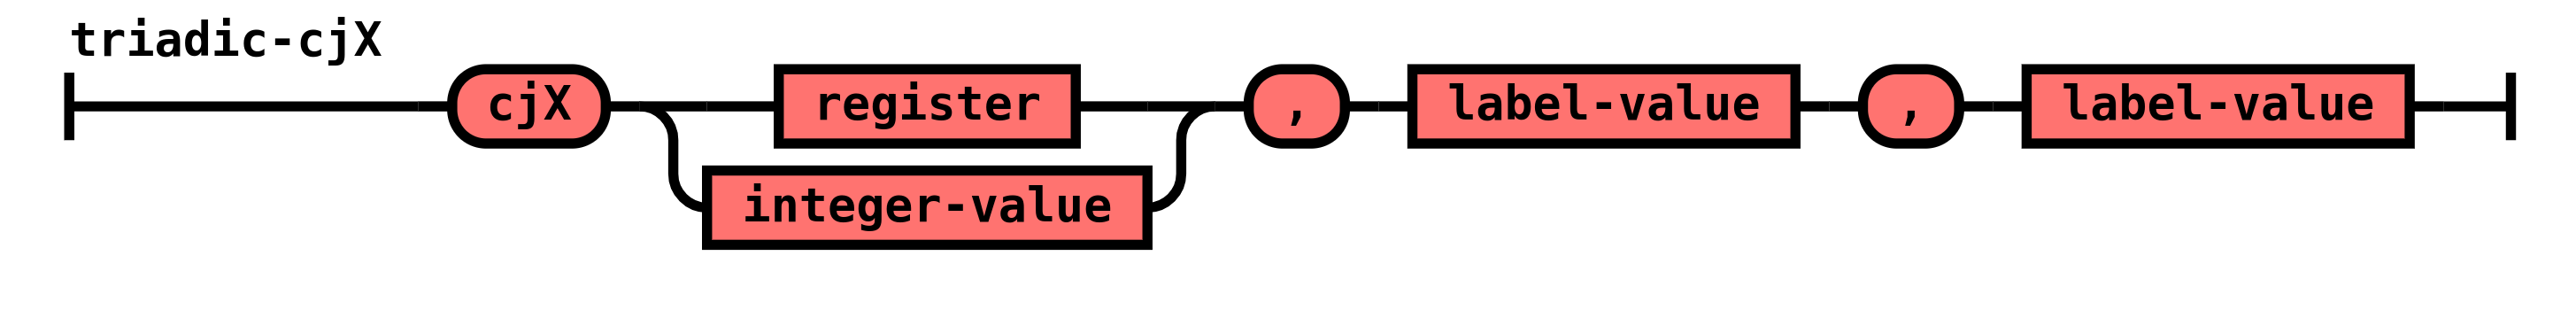
\includegraphics[width=\linewidth]{nstar/instructions/cjX-grammar}
		}
	}

	\caption{Grammar for the ternary conditional jumps.}
	\label{fig:nstar-instructionset-terminal-cjX-triadic-grammar}
\end{figure}

\begin{figure}[H]
	\centering

	\framebox[\textwidth][c]{
		\begin{prooftree}
			\hypo{\CodeTypeSequent{\Xi}{\Gamma}{\chi}{\sigma}{\epsilon}{l_1}{\Tforall{}{\Tcontext{\chi_1}{\sigma}{\epsilon}}}\hspace{1.5em}%
				\chi_1\sim\chi}
			\infer[no rule, rule margin=1.0ex]1{\CodeTypeSequent{\Xi}{\Gamma}{\chi}{\sigma}{\epsilon}{l_2}{\Tforall{}{\Tcontext{\chi_2}{\sigma}{\epsilon}}}\hspace{1.5em}%
			\chi_2\sim\chi}
			\infer[no rule, rule margin=1.0ex]1{\CodeTypeSequent{\Xi}{\Gamma}{\chi}{\sigma}{\epsilon}{a}{\Tunsigned{N}}\hspace{1em}\text{or}\hspace{1em}\CodeTypeSequent{\Xi}{\Gamma}{\chi}{\sigma}{\epsilon}{a}{\Tsigned{N}}}
			\infer1{\ISequent{\Xi}{\Gamma}{\chi}{\sigma}{\epsilon}{\IcjZ{a}{l_1}{l_2}}{\chi}{\sigma}{\epsilon}}
		\end{prooftree}
	}

	\caption{Type inference rules for the ternary conditional jumps.}
	\label{fig:nstar-instructionset-terminal-cjX-triadic-typerules}
\end{figure}

\subsubsection{Quaternary conditional jumps}\label{subsubsec:nstar-instructionset-terminal-cjX-tetradic}

Quaternary conditional jumps allow to jump to different labels depending on the relation bewteen the value of the first two parameters.
There are a few of these:
\begin{itemize}
	\item \Icje{a}{b}{m}{n}\ jumps to \texttt{m} if \texttt{a} and \texttt{b} evaluate to equal values, otherwise it jumps to \texttt{n};
	\item \Icjne{a}{b}{m}{n}\ is the same as \Icje{a}{b}{n}{m};
	\item \Icjl{a}{b}{m}{n}\ goes to \texttt{m} if \texttt{a} evaluates to a value strictly less than the value \texttt{b} evaluates to, else it goes to \texttt{n};
	\item \Icjge{a}{b}{m}{n}\ is \Icjl{b}{a}{n}{m};
	\item \Icjle{a}{b}{m}{n}\ performs the same as \Icjl{a}{b}{m}{n}\ but it also jumps to \texttt{m} if \texttt{a} evaluates to a value equal to what \texttt{b} evaluates to;
	\item \Icjg{a}{b}{m}{n}\ is exactly the same as \Icjle{b}{a}{n}{m}.
\end{itemize}
Some of them are redundant and are provided only for convenience.

All these instructions share the same grammar and type inference rules (they all are refered to as {\Iformat cjC}), present in figures~\ref{fig:nstar-instructionset-terminal-cjX-tetradic-grammar},\ref{fig:nstar-instructionset-terminal-cjX-tetradic-typerules}.

\begin{figure}[H]
	\centering

	\framebox[\textwidth][c]{
		\scalebox{.95}{
			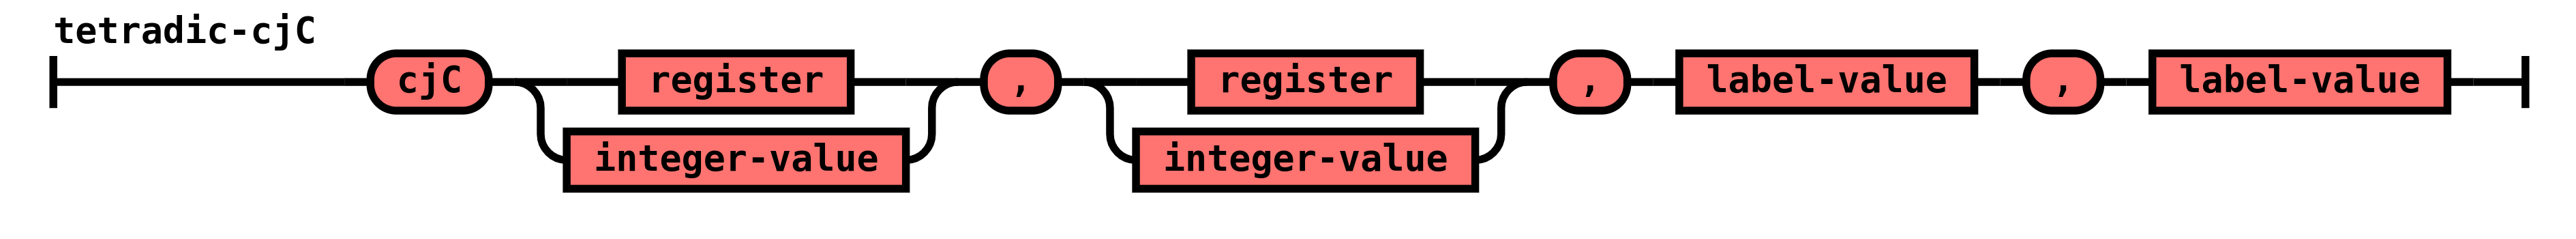
\includegraphics[width=\linewidth]{nstar/instructions/cjC-grammar}
		}
	}

	\caption{Grammar for the quaternary conditional jumps.}
	\label{fig:nstar-instructionset-terminal-cjX-tetradic-grammar}
\end{figure}

\begin{figure}[H]
	\centering

	\framebox[\textwidth][c]{
		\begin{prooftree}
			\hypo{\CodeTypeSequent{\Xi}{\Gamma}{\chi}{\sigma}{\epsilon}{l_1}{\Tforall{}{\Tcontext{\chi_1}{\sigma}{\epsilon}}}\hspace{1.5em}%
				\chi_1\sim\chi}
			\infer[no rule, rule margin=1.0ex]1{\CodeTypeSequent{\Xi}{\Gamma}{\chi}{\sigma}{\epsilon}{l_2}{\Tforall{}{\Tcontext{\chi_2}{\sigma}{\epsilon}}}\hspace{1.5em}%
			\chi_2\sim\chi}
			\infer[no rule, rule margin=1.0ex]1{\CodeTypeSequent{\Xi}{\Gamma}{\chi}{\sigma}{\epsilon}{a}{\tau_1}\hspace{1.5em}\CodeTypeSequent{\Xi}{\Gamma}{\chi}{\sigma}{\epsilon}{b}{\tau_2}\hspace{1.5em}\tau_1\iseq\tau_2}
			\infer1{\ISequent{\Xi}{\Gamma}{\chi}{\sigma}{\epsilon}{\IcjC{a}{b}{l_1}{l_2}}{\chi}{\sigma}{\epsilon}}
		\end{prooftree}
	}

	\caption{Type inference rules for the quaternary conditional jumps.}
	\label{fig:nstar-instructionset-terminal-cjX-tetradic-typerules}
\end{figure}

Type inference rules rely on a $\iseq$ binary predicate which filters whether two types can be compared (either for equality or inequality).
This is required by those instructions as values will need to be compared at runtime to choose which jump to perform.

Given $\top,\bot \in \mathbb{B}$ the symbols for boolean truth and falsity, the $\iseq$ relation can be defined as
\begin{alignat*}{4}
	 & \Tunsigned{M} \quad & \iseq & \quad \Tunsigned{N} \quad & = \top \\
	 & \Tsigned{M}   \quad & \iseq & \quad \Tsigned{N}   \quad & = \top \\
	 & \cdot         \quad & \iseq & \quad \cdot         \quad & = \bot
\end{alignat*}

\section{Stack handling instructions}\label{sec:nstar-instructionset-stack}

\subsection{\texttt{sld}}\label{subsec:nstar-instructionset-stack-sld}

The {\Iformat sld} instruction stores the value at the given index on the stack in a register.
Grammar and inference rules are given in Figure~\ref{fig:nstar-instructionset-stack-sld-grammar} and Figure~\ref{fig:nstar-instructionset-stack-sld-typerules}.

\begin{figure}[H]
	\centering

	\framebox[\textwidth][c]{
		\scalebox{.5}{
			\includegraphics{nstar/instructions/sld-grammar}
		}
	}

	\caption{Grammar for the {\Iformat sld} instruction.}
	\label{fig:nstar-instructionset-stack-sld-grammar}
\end{figure}

\begin{figure}[H]
	\centering

	\framebox[\textwidth][c]{\parbox{\textwidth}{
			\centering
			\begin{prooftree}
				\hypo{r$ is a register$}
				\hypo{n \in\mathbb{N}}
				\hypo{n \leq p}
				\infer[no rule, rule margin=1.0ex]3{\sigma= \Tsstack{t_0}{t_1}{\ldots}{t_p}{s}\hspace{1.5em}%
				t_n\sim\Tforall{}{\zeta}}
				\infer1[load cont from stack in register]{\ISequent{\Xi}{\Gamma}{\chi}{\sigma}{n}{\Isld{n}{r}}{\chi, r : t_n}{\sigma}{r}}
			\end{prooftree}
			\\\vspace{\baselineskip}
			\begin{prooftree}
				\hypo{r$ is a register$}
				\hypo{n, k \in\mathbb{N}}
				\infer[no rule, rule margin=1.0ex]2{n \leq p\hspace{1.5em}%
				k \leq 8\hspace{1.5em}%
				\sigma=\Tsstack{t_0}{t_1}{\ldots}{t_p}{s}\hspace{1.5em}%
				\KindSequent{\Gamma}{t_n}{\T{k}}}
				\infer1[load value from stack]{\ISequent{\Xi}{\Gamma}{\chi}{\sigma}{\epsilon}{\Isld{n}{r}}{\chi, r : t_n}{\sigma}{\epsilon}}
			\end{prooftree}
		}}

	\caption{Type inference rules for the {\Iformat sld} instruction.}
	\label{fig:nstar-instructionset-stack-sld-typerules}
\end{figure}

The {\Iformat sld} instruction takes two arguments: an integer and a register, and requires the integer to be a valid stack index.
The register is then bound to a value of the type at the stack index, if it can fit in it (depending on the platform, it may need to be either 8 or 4 bytes wide).
Note that it is possible to move a continuation from the stack into a register using this instruction, but overwriting the current continuation is forbidden.

\subsection{\texttt{sst}}\label{subsec:nstar-instructionset-stack-sst}

The {\Iformat sst} instruction stores a value at the given index on the stack.
Grammar and inference rules are given in Figure~\ref{fig:nstar-instructionset-stack-sst-grammar} and Figure~\ref{fig:nstar-instructionset-stack-sst-typerules}.

\begin{figure}[H]
	\centering

	\framebox[\textwidth][c]{
		\scalebox{.5}{
			\includegraphics{nstar/instructions/sst-grammar}
		}
	}

	\caption{Grammar for the {\Iformat sst} instruction.}
	\label{fig:nstar-instructionset-stack-sst-grammar}
\end{figure}

\begin{figure}[H]
	\centering

	\framebox[\textwidth][c]{\parbox{\textwidth}{
			\centering
			\begin{prooftree}
				\hypo{r$ is a register$}
				\hypo{n \in\mathbb{N}}
				\hypo{\sigma= \Tsstack{t_0}{t_1}{\ldots}{t_p}{s}}
				\infer[no rule, rule margin=1.0ex]3{n \leq p\hspace{1.5em}%
				t_n\sim\Tforall{}{\zeta}\hspace{1.5em}%
				\CodeTypeSequent{\Xi}{\Gamma}{\chi}{\sigma}{\epsilon}{r}{\Tforall{}{\zeta}}}
				\infer1[store continuation in stack]{\ISequent{\Xi}{\Gamma}{\chi}{\sigma}{r}{\Isst{r}{n}}{\chi}{\sigma}{n}}
			\end{prooftree}
			\\\vspace{\baselineskip}
			\begin{prooftree}
				\hypo{$n $\in\mathbb{N}}
				\hypo{\sigma=\Tsstack{t_0}{t_1}{\ldots}{t_p}{s}}
				\infer[no rule, rule margin=1ex]2{n \leq p\hspace{1.5em}%
				\CodeTypeSequent{\Xi}{\Gamma}{\chi}{\sigma}{\epsilon}{e}{t_n}\hspace{1.5em}%
				t_n\neq \Tbang\hspace{1.5em}%
				\epsilon \neq n}
				\infer1[store value in stack]{\ISequent{\Xi}{\Gamma}{\chi}{\sigma}{\epsilon}{\Isst{e}{n}}{\chi}{\sigma}{\epsilon}}
			\end{prooftree}
		}}


	\caption{Type inference rules for the {\Iformat sst} instruction.}
	\label{fig:nstar-instructionset-stack-sst-typerules}
\end{figure}

The {\Iformat sst} instruction takes two arguments: a register and an integer, requiring the integer to be a valid stack index pointing to a 4 or 8 bytes wide cell.
This instruction can be used to move the continuation from a register onto the stack, but overwriting the current continuation is forbidden.

\subsection{\texttt{salloc}}\label{subsec:nstar-instructionset-stack-salloc}

The {\Iformat salloc} instructions allocates some space on top of the stack for some data of the given type.
Grammar and type inference rules are given in Figure~\ref{fig:nstar-instructionset-stack-salloc-grammar} and Figure~\ref{fig:nstar-instructionset-stack-salloc-typerules}.

\begin{figure}[H]
	\centering

	\framebox[\textwidth][c]{
		\scalebox{.5}{
			\includegraphics{nstar/instructions/salloc-grammar}
		}
	}

	\caption{Grammar for the {\Iformat salloc} instruction.}
	\label{fig:nstar-instructionset-stack-salloc-grammar}
\end{figure}

\begin{figure}[H]
	\centering

	\framebox[\textwidth][c]{\parbox{\textwidth}{
			\centering
			\begin{prooftree}
				\hypo{m \in\mathbb{N}}
				\hypo{\KindSequent{\Gamma}{t}{\T{m}}}
				\hypo{\sigma^\prime=\Tstack{t}{\sigma}}
				\infer3[\texttt{salloc} with stack continuation]{\ISequent{\Xi}{\Gamma}{\chi}{\sigma}{n}{\Isalloc{t}}{\chi}{\sigma^\prime}{n+1}}
			\end{prooftree}
			\\\vspace{\baselineskip}
			\begin{prooftree}
				\hypo{m \in\mathbb{N}}
				\hypo{\KindSequent{\Gamma}{t}{\T{m}}}
				\hypo{\sigma^\prime=\Tstack{t}{\sigma}}
				\infer3{\ISequent{\Xi}{\Gamma}{\chi}{\sigma}{\epsilon}{\Isalloc{t}}{\chi}{\sigma^\prime}{\epsilon}}
			\end{prooftree}
		}}

	\caption{Type inference rules for the {\Iformat salloc} instruction.}
	\label{fig:nstar-instructionset-stack-salloc-typerules}
\end{figure}

The {\Iformat salloc} instruction allows reserving (allocating) $n$ bytes of memory on top of the stack, for a specific type which is $n$ bytes wide.
Note that according to the {\Iformat sst} instruction, the type may be changed later on.
If the continuation is currently on the stack, then it is shifted one cell to the right (its stack index is incremented by 1).

\subsection{\texttt{sfree}}\label{subsec:nstar-instructionset-stack-sfree}

The {\Iformat sfree} instruction frees the top-most stack cell.
Grammar and type inference rules are respectively given in Figure~\ref{fig:nstar-instructionset-stack-sfree-grammar} and Figure~\ref{fig:nstar-instructionset-stack-sfree-typerules}.

\begin{figure}[H]
	\centering

	\framebox[\textwidth][c]{
		\scalebox{.5}{
			\includegraphics{nstar/instructions/sfree-grammar}
		}
	}

	\caption{Grammar for the {\Iformat sfree} instruction.}
	\label{fig:nstar-instructionset-stack-sfree-grammar}
\end{figure}

\begin{figure}[H]
	\centering

	\framebox[\textwidth][c]{\parbox{\textwidth}{
			\centering
			\begin{prooftree}
				\hypo{1 \leq n \leq p}
				\hypo{\sigma=\Tsstack{t_0}{t_1}{\ldots}{t_p}{s}}
				\hypo{\sigma^\prime=\Tsstack{t_1}{\ldots}{t_p}{s}}
				\infer3[\texttt{sfree} with stack continuation]{\ISequent{\Xi}{\Gamma}{\chi}{\sigma}{n}{\Isfree}{\chi}{\sigma^\prime}{n-1}}
			\end{prooftree}
			\\\vspace{\baselineskip}
			\begin{prooftree}
				\hypo{\sigma=\sigma=\Tsstack{t_0}{t_1}{\ldots}{t_p}{s}}
				\hypo{\sigma^\prime=\Tsstack{t_1}{\ldots}{t_p}{s}}
				\infer2{\ISequent{\Xi}{\Gamma}{\chi}{\sigma}{\epsilon}{\Isfree}{\chi}{\sigma^\prime}{\epsilon}}
			\end{prooftree}
		}}

	\caption{Type inference rules for the {\Iformat sfree} instruction.}
	\label{fig:nstar-instructionset-stack-sfree-typerules}
\end{figure}

The {\Iformat sfree} instruction frees the top-most stack cell available unless it contains the current continuation.
If not, the continuation is shifted left (its stack index is decremented by 1).
Note that freeing a stack cell does not mean all the pointers to it are invalidated, nor that the memory occupied is zeroed out.
Accessing old references to it is considered Undefined Behavior, and is therefore unreliable.

\subsection{\texttt{sref}}\label{subsec:nstar-instructionset-stack-sref}

The {\Iformat sref} instruction fetches a pointer (to be used by memory instructions) to some data available on the stack.
This can be used to construct references to e.g.\ stack-allocated structures (which cannot be written to nor read from otherwise).
The grammar and inference rules are given respectively in Figure~\ref{fig:nstar-instructionset-stack-sref-grammar} and Figure~\ref{fig:nstar-instructionset-stack-sref-typerules}.

\begin{figure}[H]
	\centering

	\framebox[\textwidth][c]{
		\scalebox{.5}{
			\includegraphics{nstar/instructions/sref-grammar}
		}
	}

	\caption{Grammar for the {\Iformat sref} instruction.}
	\label{fig:nstar-instructionset-stack-sref-grammar}
\end{figure}

\begin{figure}[H]
	\centering

	\framebox[\textwidth][c]{
		\parbox{\textwidth}{
			\centering

			\begin{prooftree}
				\hypo{r$ is a register$}
				\hypo{n \in\mathbb{N}}
				\hypo{n \leq p}
				\infer[no rule, rule margin=1ex]3{\sigma=\Tsstack{t_0}{t_1}{\ldots}{t_p}{s}\hspace{1.5em}%
				t_n\nsim \Tbang\hspace{1.5em}%
				t_n\nsim \Tforall{}{\zeta}\hspace{1.5em}%
				\epsilon\neq n}
				\infer1{\ISequent{\Xi}{\Gamma}{\chi}{\sigma}{\epsilon}{\Isref{n}{r}}{\chi, r : \Tptr{t_n}}{\sigma}{\epsilon}}
			\end{prooftree}
		}
	}

	\caption{Type inference rules for the {\Iformat sref} instruction.}
	\label{fig:nstar-instructionset-stack-sref-typerules}
\end{figure}

The {\Iformat sref} instruction takes an integer and a register as arguments, and requires the integer to be a valid stack index to a type at most 4 or 8 bytes wide.
For security reasons, it is forbidden to take a reference to a bang-type (which is unsized) or to a function pointer, as it could lead to duplicating a continuation.

Note that trying to write to a pointer to stack data which has been freed with {\Iformat sfree} (as in Listing~\ref{lst:nstar-instructionset-stack-sref-ubexample}) is Undefined Behavior.
This is something that we cannot check (it could be possible with linear types) in \nstar\ because it goes beyond the type system described in this document.

\begin{listing}[H]
	\centering
	\inputminted{\nstarlexer}{examples/sref-undefined-behavior.nst}

	\caption{An undefined behavior triggered through the use of {\Iformat sref}.}
	\label{lst:nstar-instructionset-stack-sref-ubexample}
\end{listing}

\section{Memory handling instructions}\label{sec:nstar-instructionset-memory}

Memory instructions are instructions which can only operate on pointers to data.
Those may be used to access data in the \texttt{data} sections or even \texttt{malloc}ed data.

\subsection{\texttt{ld}}\label{subsec:nstar-instructionset-memory-ld}

The {\Iformat ld} instruction loads a value from a memory area into a register.
Grammar and inference rules are given in Figure~\ref{fig:nstar-instructionset-memory-ld-grammar} and Figure~\ref{fig:nstar-instructionset-memory-ld-typerules}.

\begin{figure}[H]
	\centering

	\framebox[\textwidth][c]{
		\scalebox{.5}{
			\includegraphics{nstar/instructions/ld-grammar}
		}
	}

	\caption{Grammar for the {\Iformat ld} instruction.}
	\label{fig:nstar-instructionset-memory-ld-grammar}
\end{figure}

\begin{figure}[H]
	\centering

	\framebox[\textwidth][c]{\parbox{\textwidth}{
			\centering
			\begin{prooftree}
				\hypo{r$ is a register$}
				\hypo{r \neq\epsilon}
				\hypo{\CodeTypeSequent{\Xi}{\Gamma}{\chi}{\sigma}{\epsilon}{\Ebyteoff{o}{p}}{\Tptr{t}}}
				\infer3[load value from pointer byte offset]{\ISequent{\Xi}{\Gamma}{\chi}{\sigma}{\epsilon}{\Ild{\Ebyteoff{o}{p}}{r}}{\chi, r : t}{\sigma}{\epsilon}}
			\end{prooftree}
			\\\vspace{\baselineskip}
			\begin{prooftree}
				\hypo{r$ is a register$}
				\hypo{r \neq\epsilon}
				\hypo{\CodeTypeSequent{\Xi}{\Gamma}{\chi}{\sigma}{\epsilon}{\Ebaseoff{p}{o}}{\Tptr{t}}}
				\infer3[load value from pointer base offset]{\ISequent{\Xi}{\Gamma}{\chi}{\sigma}{\epsilon}{\Ild{\Ebaseoff{p}{o}}{r}}{\chi, r : t}{\sigma}{\epsilon}}
			\end{prooftree}
		}}

	\caption{Type inference rules for the {\Iformat ld} instruction.}
	\label{fig:nstar-instructionset-memory-ld-typerules}
\end{figure}

The {\Iformat ld} instruction takes a register and a pointer offset as arguments, and requires that the value held in the register matches the value behind the pointer.
This instruction does not allow overwriting the current continuation, if stored in the register passed as argument.

\subsection{\texttt{st}}\label{subsec:nstar-instructionset-memory-st}

The {\Iformat st} instruction stores a value into a memory area denoted by pointer offset.
The grammar and inference rules are given in Figure~\ref{fig:nstar-instructionset-memory-st-grammar} and Figure~\ref{fig:nstar-instructionset-memory-st-typerules}.

\begin{figure}[H]
	\centering

	\framebox[\textwidth][c]{
		\scalebox{.5}{
			\includegraphics{nstar/instructions/st-grammar}
		}
	}

	\caption{Grammar for the {\Iformat st} instruction.}
	\label{fig:nstar-instructionset-memory-st-grammar}
\end{figure}

\begin{figure}[H]
	\centering

	\framebox[\textwidth][c]{\parbox{\textwidth}{
			\centering
			\begin{prooftree}
				\hypo{\CodeTypeSequent{\Xi}{\Gamma}{\chi}{\sigma}{\epsilon}{e}{t}}
				\infer[no rule, rule margin=1ex]1{e \neq\epsilon\hspace{1.5em}
				t \neq \Tbang\hspace{1.5em}
				\CodeTypeSequent{\Xi}{\Gamma}{\chi}{\sigma}{\epsilon}{\Ebyteoff{o}{p}}{\Tptr{t}}}
				\infer1[store value in pointer byte offset]{\ISequent{\Xi}{\Gamma}{\chi}{\sigma}{\epsilon}{\Ist{e}{\Ebyteoff{o}{p}}}{\chi}{\sigma}{\epsilon}}
			\end{prooftree}
			\\\vspace{\baselineskip}
			\begin{prooftree}
				\hypo{\CodeTypeSequent{\Xi}{\Gamma}{\chi}{\sigma}{\epsilon}{e}{t}}
				\infer[no rule, rule margin=1ex]1{e \neq\epsilon\hspace{1.5em}
				t \neq \Tbang\hspace{1.5em}
				\CodeTypeSequent{\Xi}{\Gamma}{\chi}{\sigma}{\epsilon}{\Ebaseoff{p}{o}}{\Tptr{t}}}
				\infer1[store value in pointer base offset]{\ISequent{\Xi}{\Gamma}{\chi}{\sigma}{\epsilon}{\Ist{e}{\Ebaseoff{p}{o}}}{\chi}{\sigma}{\epsilon}}
			\end{prooftree}
		}}

	\caption{Type inference rules for the {\Iformat st} instruction.}
	\label{fig:nstar-instructionset-memory-st-typerules}
\end{figure}

The {\Iformat st} instruction takes a value (literal value or register) and a pointer offset as arguments.
If a register is passed, it cannot contain the current continuation.
Note that the value is not moved from the register, it is simply copied into the pointer.
The register must also not hold a value of unknown type $\Tbang$, because its type is not known.

\section{Register handling instructions}\label{sec:nstar-instructionset-registers}

\subsection{\texttt{mv}}\label{subsec:nstar-instructionset-registers-mv}

The {\Iformat mv} instruction moves a value (immediate value or stored in a register) into a register.
Grammar is given in Figure~\ref{fig:nstar-instructionset-registers-mv-grammar}.
Type inference rules are given in Figure~\ref{fig:nstar-instructionset-registers-mv-typerules}.

\begin{figure}[H]
	\centering

	\framebox[\textwidth][c]{
		\scalebox{.5}{
			\includegraphics{nstar/instructions/mov-grammar}
		}
	}

	\caption{Grammar of the {\Iformat mv} instruction.}
	\label{fig:nstar-instructionset-registers-mv-grammar}
\end{figure}

\begin{figure}[H]
	\centering

	\framebox[\textwidth][c]{\parbox{\textwidth}{
			\centering
			\begin{prooftree}
				\hypo{r, d$ are registers$}
				\hypo{\CodeTypeSequent{\Xi}{\Gamma}{\chi}{\sigma}{\epsilon}{r}{\Tforall{}{\zeta}}}
				\infer2[move cont from register to register]{\ISequent{\Xi}{\Gamma}{\chi}{\sigma}{r}{\Imv{r}{d}}{\chi\setminus\{r\}, d : \Tforall{}{\zeta}}{\sigma}{d}}
			\end{prooftree}
			\\\vspace{\baselineskip}
			\begin{prooftree}
				\hypo{r$ is a register$}
				\hypo{n \leq 8}
				\infer[no rule, rule margin=1ex]2{\KindSequent{\Gamma}{t}{\T{n}}\hspace{1.5em}
				\CodeTypeSequent{\Xi}{\Gamma}{\chi}{\sigma}{\epsilon}{e}{t}\hspace{1.5em}
				t \neq \Tbang}
				\infer1[move value to register]{\ISequent{\Xi}{\Gamma}{\chi}{\sigma}{\epsilon}{\Imv{e}{r}}{\chi\setminus\{r\}, r : t}{\sigma}{\epsilon}}
			\end{prooftree}
		}}

	\caption{Type inference rules for the {\Iformat mv} instruction.}
	\label{fig:nstar-instructionset-registers-mv-typerules}
\end{figure}

The {\Iformat mv} instruction takes a value (literal value or register) and a register as arguments, and overwrites the second register with a copy of the first value (if in a register).
The value in the first register is not discarded.
This instruction can be used to \textit{move} the continuation from one register to another, in which case no copy is performed (the function pointer is moved, to prevent from duplicating the continuation).
If the first argument is a register, then it cannot be bound to a bang-type.

\subsection{Logical instructions}\label{subsec:nstar-instructionset-registers-logical}

There are two kinds of logical instructions:
\begin{itemize}
	\item Unary instructions, such as {\Iformat not}, which take two parameters: one source operand and a destination;
	\item Binary instructions, such as {\Iformat and}, which take three parameters: two source operands and a destination;
	\item Logical shifts.
\end{itemize}
All the instructions within each group share the same grammar and type inference rules.

\subsubsection{Unary logical instructions}\label{subsubsec:nstar-instructionset-registers-logical-unary}

Unary logical instructions take a single parameter, perform some operation on it and store their result in their destination operand.
Here is a complete list of all unary logical instructions:
\begin{itemize}
	\item \Inot{a}{r}\ which performs one's complement negation (basically bit flipping, meaning that $0 \mapsto 1$ and $1 \mapsto 0$ for every bit) on \texttt{a} and stores the result in \texttt{r}.
\end{itemize}
Grammar and type inference rules are presented in figures~\ref{fig:nstar-instructionset-registers-logical-unary-grammar},\ref{fig:nstar-instructionset-registers-logical-unary-typerules}.

\begin{figure}[H]
	\centering

	\framebox[\textwidth][c]{
		\scalebox{.8}{
			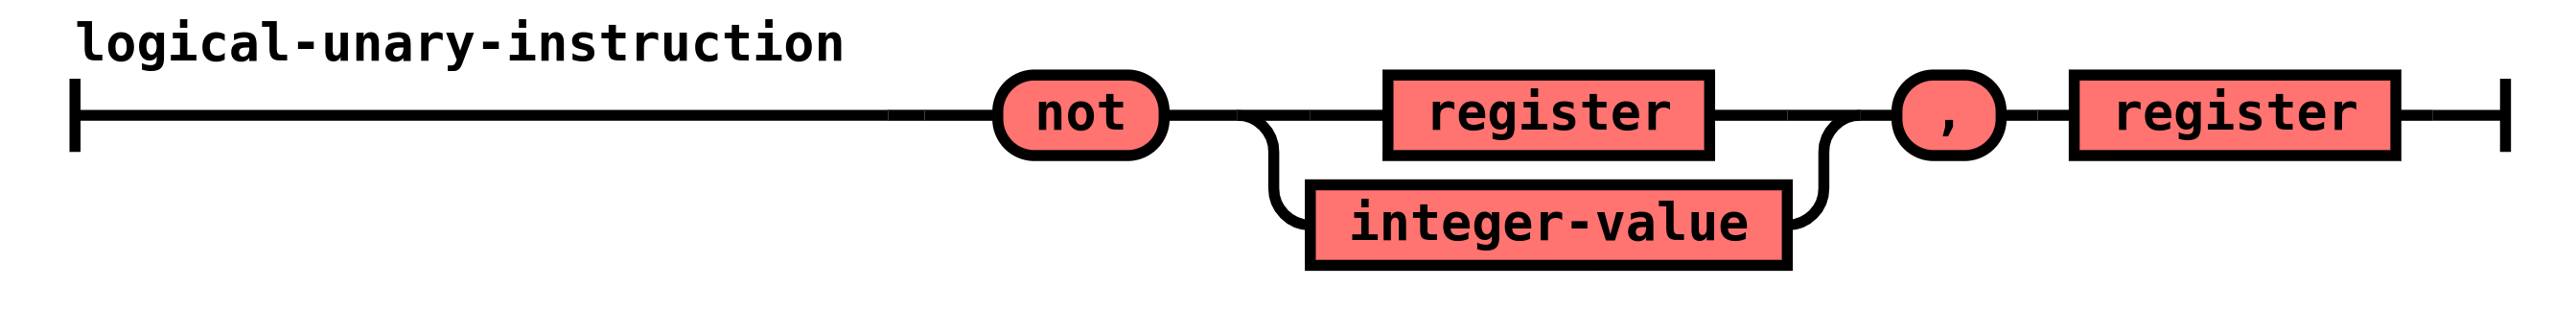
\includegraphics[width=\linewidth]{nstar/instructions/logical1-grammar}
		}
	}

	\caption{Grammar for unary logical instructions.}
	\label{fig:nstar-instructionset-registers-logical-unary-grammar}
\end{figure}

\begin{figure}[H]
	\centering

	\framebox[\textwidth][c]{
		\begin{prooftree}
			\hypo{\CodeTypeSequent{\Xi}{\Gamma}{\chi}{\sigma}{\epsilon}{x}{\tau}}
			\hypo{r$ is a register$}
			\hypo{r \neq \epsilon}
			\hypo{\tau\in\{\Tunsigned{N}, \Tsigned{N}\}}
			\infer4{\ISequent{\Xi}{\Gamma}{\chi}{\sigma}{\epsilon}{\Inot{x}{r}}{\chi, r : \tau}{\sigma}{\epsilon}}
		\end{prooftree}
	}

	\caption{Type inference rules for unary logical instructions.}
	\label{fig:nstar-instructionset-registers-logical-unary-typerules}
\end{figure}

\subsubsection{Binary logical instructions}\label{subsubsec:nstar-instructionset-registers-logical-binary}

Binary logical instructions take three parameters, two of which are combined bit by bit following the truch tables given in table~\ref{table:nstar-instructionset-registers-logical-binary-truthtables}.
The result is stored in the third operand (the destination operand).

\begin{table}[H]
	\hspace*{\fill}%
	\begin{tabularx}{0.25\linewidth}{ccY}
		\toprule
		a & b & a~{\Iformat and}~b \\
		\midrule
		0 & 0 & 0                  \\
		0 & 1 & 0                  \\
		1 & 0 & 0                  \\
		1 & 1 & 1                  \\
		\bottomrule
	\end{tabularx}\hspace*{\fill}%
	\begin{tabularx}{0.25\linewidth}{ccY}
		\toprule
		a & b & a~{\Iformat or}~b \\
		\midrule
		0 & 0 & 0                 \\
		0 & 1 & 1                 \\
		1 & 0 & 1                 \\
		1 & 1 & 1                 \\
		\bottomrule
	\end{tabularx}\hspace*{\fill}%
	\begin{tabularx}{0.25\linewidth}{ccY}
		\toprule
		a & b & a~{\Iformat xor}~b \\
		\midrule
		0 & 0 & 0                  \\
		0 & 1 & 1                  \\
		1 & 0 & 1                  \\
		1 & 1 & 0                  \\
		\bottomrule
	\end{tabularx}%
	\hspace*{\fill}

	\caption{Truth table for all the logical binary instructions.}
	\label{table:nstar-instructionset-registers-logical-binary-truthtables}
\end{table}

Grammar and type inference rules are given (for any logical binary instruction) in figures~\ref{fig:nstar-instructionset-registers-logical-binary-grammar},\ref{fig:nstar-instructionset-registers-logical-binary-typerules}.

\begin{figure}[H]
	\centering

	\framebox[\textwidth][c]{
		\scalebox{.9}{
			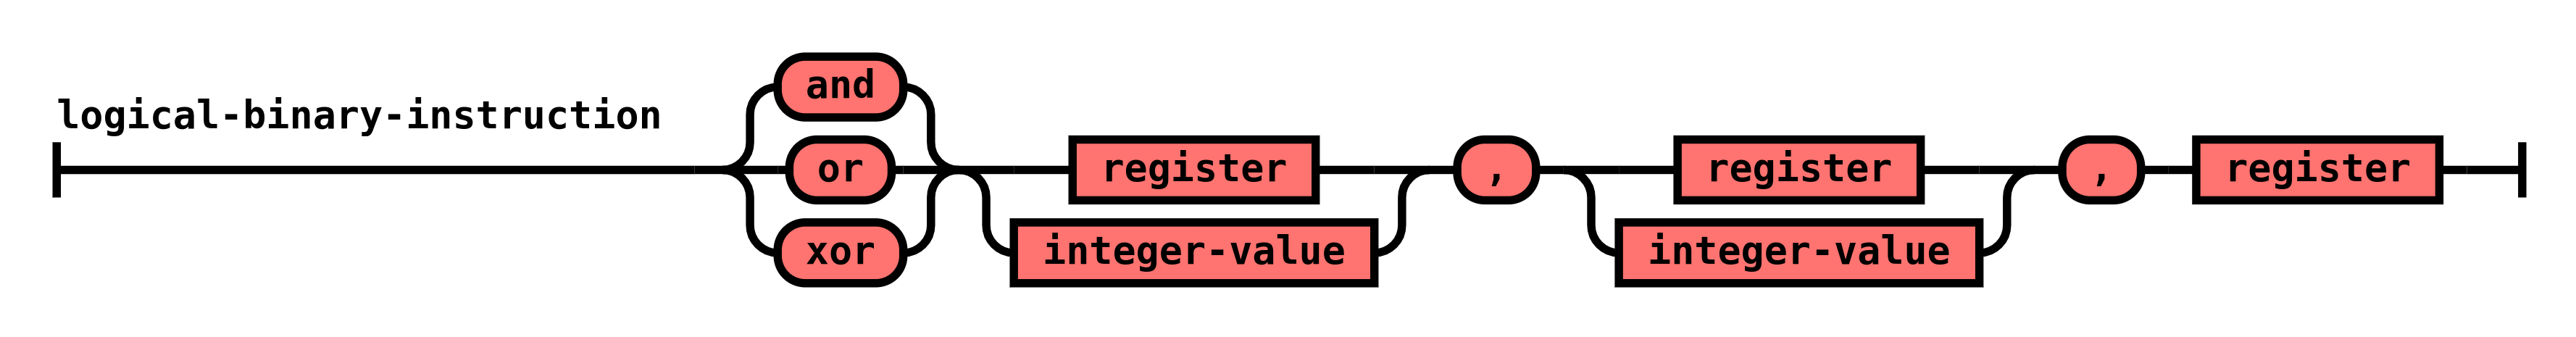
\includegraphics[width=\linewidth]{nstar/instructions/logical2-grammar}
		}
	}

	\caption{Grammar for binary logical instructions.}
	\label{fig:nstar-instructionset-registers-logical-binary-grammar}
\end{figure}

\begin{figure}[H]
	\centering

	\framebox[\textwidth][c]{
		\begin{prooftree}
			\hypo{r$ is a register$}
			\hypo{r \neq \epsilon}
			\infer[no rule, rule margin=1ex]2{%
			\CodeTypeSequent{\Xi}{\Gamma}{\chi}{\sigma}{\epsilon}{x}{\tau}\hspace{1.5em}%
			\CodeTypeSequent{\Xi}{\Gamma}{\chi}{\sigma}{\epsilon}{y}{\tau}\hspace{1.5em}%
			\tau\in\{\Tunsigned{N}, \Tsigned{N}\}%
			}
			\infer1{\ISequent{\Xi}{\Gamma}{\chi}{\sigma}{\epsilon}{\Iand{x}{y}{r}}{\chi, r : \tau}{\sigma}{\epsilon}}
		\end{prooftree}
	}

	\caption{Type inference rules for binary logical instructions.}
	\label{fig:nstar-instructionset-registers-logical-binary-typerules}
\end{figure}


\subsubsection{Logical shifts}\label{subsubsec:nstar-instructionset-registers-logical-shifts}

Despite being binary logical instructions, logical shifts do not quite share the same grammar as other instructions such as {\Iformat and}, because the second argument is required to be a literal integer.
Type inference rules will therefore also be different (although very similar).
These two are presented in figures~\ref{fig:nstar-instructionset-registers-logical-shifts-grammar},\ref{fig:nstar-instructionset-registers-logical-shifts-typerules}.

\begin{figure}[H]
	\centering

	\framebox[\textwidth][c]{
		\scalebox{.8}{
			\includegraphics[width=\linewidth]{nstar/instructions/shiftX-grammar}
		}
	}

	\caption{Grammar for logical shifts.}
	\label{fig:nstar-instructionset-registers-logical-shifts-grammar}
\end{figure}

\begin{figure}[H]
	\centering

	\framebox[\textwidth][c]{
		\begin{prooftree}
			\hypo{\CodeTypeSequent{\Xi}{\Gamma}{\chi}{\sigma}{\epsilon}{x}{\tau}}
			\hypo{r$ is a register$}
			\hypo{r \neq \epsilon}
			\hypo{\tau\in\{\Tunsigned{N}, \Tsigned{N}\}}
			\infer4{\ISequent{\Xi}{\Gamma}{\chi}{\sigma}{\epsilon}{\IshiftX{x}{n}{r}}{\chi, r : \tau}{\sigma}{\epsilon}}
		\end{prooftree}
	}

	\caption{Type inference rules for logical shifts.}
	\label{fig:nstar-instructionset-registers-logical-shifts-typerules}
\end{figure}

\subsection{Conditional moves}\label{subsec:nstar-instructionset-registers-cmvX}

Conditional moves come in two different batches:
\begin{itemize}
	\item Quaternary conditional moves, taking only one parameter for the condition;
	\item Quintary conditional moves, taking two parameters for the condition.
\end{itemize}
Each category uses the same grammar and type inference rules for every instruction within.

\subsubsection{Quaternary conditional moves}\label{subsubsec:nstar-instructionset-registers-cmvX-quaternary}

There are two kinds of quaternary conditional moves:
\begin{itemize}
	\item \Icmvz{a}{b}{c}{r}\ which acts as \Imv{b}{r}\ if \texttt{a} evaluates to \texttt{0} else as \Imv{c}{r};
	\item \Icmvnz{a}{b}{c}{r}\ which is exactly the same as \Icmvz{a}{c}{b}{r}\ (it is \Imv{b}{r}\ if \texttt{a} evaluates to \texttt{0} else \Imv{c}{r}).
\end{itemize}

These instructions are so similar that they share their grammar and type inference rules, as described in figures~\ref{fig:nstar-instructionset-registers-cmvX-quaternary-grammar},\ref{fig:nstar-instructionset-registers-cmvX-quaternary-typerules}.

\begin{figure}[H]
	\centering

	\framebox[\textwidth][c]{
		\scalebox{.9}{
			\includegraphics[width=\linewidth]{nstar/instructions/cmvZ-grammar}
		}
	}

	\caption{Grammar for quaternary conditional move instructions.}
	\label{fig:nstar-instructionset-registers-cmvX-quaternary-grammar}
\end{figure}

\begin{figure}[H]
	\centering

	\framebox[\textwidth][c]{
		\begin{prooftree}
			\hypo{\CodeTypeSequent{\Xi}{\Gamma}{\chi}{\sigma}{\epsilon}{a}{\tau_1}}
			\hypo{\tau_1 \in\{ \Tunsigned{N}, \Tsigned{N} \}}
			\infer[no rule, rule margin=1ex]2{\CodeTypeSequent{\Xi}{\Gamma}{\chi}{\sigma}{\epsilon}{b}{\tau_2}\hspace{1.5em}%
			\CodeTypeSequent{\Xi}{\Gamma}{\chi}{\sigma}{\epsilon}{c}{\tau_2}\hspace{1.5em}%
			r \neq \epsilon \wedge b \neq \epsilon \wedge c \neq \epsilon}
			\infer1{\ISequent{\Xi}{\Gamma}{\chi}{\sigma}{\epsilon}{\IcmvZ{a}{b}{c}{r}}{\chi, r : \tau_2}{\sigma}{\epsilon}}
		\end{prooftree}
	}

	\caption{Type inference rules for quaternary conditional move instructions.}
	\label{fig:nstar-instructionset-registers-cmvX-quaternary-typerules}
\end{figure}

\subsubsection{Quintary conditional moves}\label{subsubsec:nstar-instructionset-registers-cmvX-quintary}

Quintary conditional move instructions come in multiple flavors:
\begin{itemize}
	\item \Icmve{a}{b}{c}{d}{r}\ performs \Imv{c}{r}\ if \texttt{a} and \texttt{b} evaluate to the same value otherwise it performs \Imv{d}{r};
	\item \Icmvne{a}{b}{c}{d}{r}\ is just the same as \Icmve{a}{b}{d}{c}{r};
	\item \Icmvl{a}{b}{c}{d}{r}\ is reduced to \Imv{c}{r}\ if \texttt{a} is reduced to a value which is stricly less than the value into which \texttt{b} is reduced, else it is reduced to \Imv{d}{r};
	\item \Icmvge{a}{b}{c}{d}{r}\ is the dual of {\Iformat cmvl}, and can be reduced to simply \Icmvl{b}{a}{d}{c}{r};
	\item \Icmvle{a}{b}{c}{d}{r}\ is very similar to \Icmvl{a}{b}{c}{d}{r}\ but it also performs \Imv{c}{r}\ if \texttt{a} and \texttt{a} are reduced to the same value;
	\item \Icmvg{a}{b}{c}{d}{r}\ is the same as \Icmvle{b}{a}{d}{c}{r}.
\end{itemize}

Grammar and type inference rules for these instructions are provided in the figures~\ref{fig:nstar-instructionset-registers-cmvX-quintary-grammar},\ref{fig:nstar-instructionset-registers-cmvX-quintary-typerules}.

\begin{figure}[H]
	\centering

	\framebox[\textwidth][c]{
		\scalebox{.9}{
			\includegraphics[width=\linewidth]{nstar/instructions/cmvX-grammar}
		}
	}

	\caption{Grammar for quintary conditional move instructions.}
	\label{fig:nstar-instructionset-registers-cmvX-quintary-grammar}
\end{figure}

\begin{figure}[H]
	\centering

	\framebox[\textwidth][c]{
		\begin{prooftree}
			\hypo{\CodeTypeSequent{\Xi}{\Gamma}{\chi}{\sigma}{\epsilon}{a}{\tau_1}}
			\hypo{\CodeTypeSequent{\Xi}{\Gamma}{\chi}{\sigma}{\epsilon}{b}{\tau_2}}
			\hypo{\tau_1\iseq\tau_2}
			\infer[no rule, rule margin=1ex]3{\CodeTypeSequent{\Xi}{\Gamma}{\chi}{\sigma}{\epsilon}{c}{\tau_3}\hspace{1.5em}%
			\CodeTypeSequent{\Xi}{\Gamma}{\chi}{\sigma}{\epsilon}{d}{\tau_3}\hspace{1.5em}%
			r \neq \epsilon \wedge c \neq \epsilon \wedge d \neq \epsilon}
			\infer1{\ISequent{\Xi}{\Gamma}{\chi}{\sigma}{\epsilon}{\IcmvC{a}{b}{c}{d}{r}}{\chi, r : \tau_3}{\sigma}{\epsilon}}
		\end{prooftree}
	}

	\caption{Type inference rules for quintary conditional move instructions.}
	\label{fig:nstar-instructionset-registers-cmvX-quintary-typerules}
\end{figure}


\section{Other instructions}\label{sec:nstar-instructionset-other}

\subsection{\texttt{nop}}\label{subsec:nstar-instructionset-other-nop}

The {\Iformat nop} instruction does absolutely nothing else than skipping a CPU cycle and taking space in the end executable.
Grammar and type inference rules are respectively given in Figure~\ref{fig:nstar-instructionset-other-nop-grammar} and Figure~\ref{fig:nstar-instructionset-other-nop-typerules}.

\begin{figure}[H]
	\centering

	\framebox[\textwidth][c]{
		\scalebox{.5}{
			\includegraphics{nstar/instructions/nop-grammar}
		}
	}

	\caption{Grammar for the {\Iformat nop} instruction.}
	\label{fig:nstar-instructionset-other-nop-grammar}
\end{figure}

\begin{figure}[H]
	\centering

	\framebox[\textwidth][c]{
		\begin{prooftree}
			\infer0{\ISequent{\Xi}{\Gamma}{\chi}{\sigma}{\epsilon}{\Inop}{\chi}{\sigma}{\epsilon}}
		\end{prooftree}
	}

	\caption{Type inference rules for the {\Iformat nop} instruction.}
	\label{fig:nstar-instructionset-other-nop-typerules}
\end{figure}

\chapter{Target-dependent features}\label{chap:nstar-specific}

\section{x86, amd64}\label{sec:nstar-specific-x86amd64}

\subsection{Register mappings}\label{subsec:nstar-specific-x86amd64-registers}

\begin{tabularx}{\textwidth}{Y Y Y}
	\toprule
	\nstar & x86 & amd64 \\
	\midrule
	r0     & eax & rax   \\
	r1     & ecx & rcx   \\
	r2     & edx & rdx   \\
	r3     & ebx & rbx   \\
	r4     & esi & rsi   \\
	r5     & edi & rdi   \\
	\bottomrule
\end{tabularx}

\chapter{The NSAM}\label{chap:nstar-nsam}

\usingnamespace{nsam}

The \nstar\ abstract machine (``NSAM'' for short) is a computation model for low-level assembly languages, especially \nstar.
Its core is untyped and may yield undefined behavior when used incorrectly.
However, in the context of \nstar, the core of the NSAM does not need to be type-safe because \nstar\ already is.

This abstract machine describes the operational semantics of the NSAM core, which is a subset of the instructions available in \nstar.
But some instructions like \texttt{call} may be encoded using the defined primitives below.
A rough translation of some \nstar\ instructions will be proposed as a simple beginning point in Figure~\ref{fig:nstar-nsam-translation-nstar-nsam}, but this is by no mean meant to be an exhaustive list of the possible translations.

\begin{figure}[htb]
	\centering

	\framebox[\textwidth][c]{
		\begin{tabular}{*{3}{>{\centering\arraybackslash}p{0.30\textwidth}}}
			$\_;\_;\_\vdash\Ijmp{l\Tunion{\vec{t}}} \rightsquigarrow \text{\Injmp{l}}$          &
			$\_;\_;\_\vdash\Icall{l\Tunion{\vec{t}}} \rightsquigarrow \text{\Injmp{l}}$         &
			$\_;\_;r\vdash\Iret \rightsquigarrow \text{\Injmp{r}}$                                           \\

			\rule{0pt}{1ex}                                                                                  \\

			$\_;\_;\_\vdash\Isalloc{t} \rightsquigarrow \text{\Insalloc{sizeof(t)}}$            &
			$\_;\Tstack{t}{\sigma};\_\vdash\Isfree \rightsquigarrow \text{\Insfree{sizeof(t)}}$ &
			$\_;\_;\_\vdash\Ihalt \rightsquigarrow \text{\Inhalt}$                                           \\

			\rule{0pt}{1ex}                                                                                  \\

			                                                                                    & $\ldots$ &
		\end{tabular}
	}

	\caption{The beginning of a small translation model from \nstar\ to the NSAM core. \textbf{$\chi;\sigma;\epsilon\vdash\text{i} \rightsquigarrow \textit{i}$} is the translation from the \nstar\ typed instruction \textbf{$\chi;\sigma;\epsilon\vdash\text{i}$} into the NSAM core instruction \textbf{$\textit{i}$}.}
	\label{fig:nstar-nsam-translation-nstar-nsam}
\end{figure}

\section{Core instructions}\label{sec:nstar-nsam-core}

The NSAM is composed of several core instructions which all form a subset of the available instructions in \nstar.
These instructions are described in Figure~\ref{fig:nstar-nsam-core-instructions}.

\begin{longtable}[H]{p{0.45\textwidth}p{0.45\textwidth}}
	\toprule
	Instruction                     & Description                                                                                                             \\
	\midrule \endhead
	\Injmp{l}                       & Transfers the control flow to the code address pointed by the label \texttt{l}                                          \\
	\Injmp{r}                       & Transfers the control flow to the code address stored in the register \texttt{r}                                        \\
	\Incjmp{cc}{a}{b}{l$_1$}{l$_2$} & Transfers the control flow to the code address pointed by the label \texttt{l$_1$} if $\texttt{cc(a, b)}=\top$.
	Otherwise, it transfers the control flow to the code address pointed by the label \texttt{l$_2$}.                                                         \\
	\Insalloc{n}                    & Allocates a space of \texttt{n} bytes on top of the stack                                                               \\
	\Insfree{n}                     & Pops a space of \texttt{n} bytes off the top of the stack                                                               \\
	\Inhalt                         & Stops the execution of code by emptying the code buffer                                                                 \\
	\Inmv{s}{d}                     & Moves a value (either a literal value or a value taken from a register) into the destination register \texttt{d}        \\
	\Insld{n}{s}{r}                 & Copies \texttt{s} bytes taken \texttt{n} bytes from the top of the stack into the register \texttt{r}                   \\
	\Insst{r}{n}                    & Copies the value in the register \texttt{r} to \texttt{n} bytes from the top of the stack                               \\
	\Inld{o}{p}{s}{r}               & Copies \texttt{s} bytes at the address \texttt{p + o} into the register \texttt{r}                                      \\
	\Inst{r}{o}{p}                  & Copies the value in the register \texttt{r} into the memory space at the address \texttt{p + o}                         \\
	\Insref{n}{p}{r}                & Retrieves a pointer to \texttt{p} bytes long data located at \texttt{n} bytes onto the stack in the register \texttt{r} \\
	\bottomrule

	\caption{The core instructions of the NSAM along with a small description of each one of them.}
	\label{fig:nstar-nsam-core-instructions}
\end{longtable}

\section{Operational semantics}\label{sec:nstar-nsam-opsem}

This section describes the operational semantics of the core instructions described in Section~\ref{sec:nstar-nsam-core}~``\nameref{sec:nstar-nsam-core}''.
It contains some specific notation as described below:
\begin{itemize}
	\item A state $S$ is a triplet $\Enstate{H}{\chi}{\sigma}$ containing:
	      \begin{itemize}
		      \item the heap $H$, which itself is the union of $\HD$ and $\HC$, respectively the global data heap and the global code heap;
		      \item the set of register bound $\chi$, associated to their respective values. The empty set is denoted $\cdot$, and union of two sets is denoted using the usual $\cup$;
		      \item the current stack $\sigma$, which is either the empty stack $\cdot$ or the stack composed of an element of size $n$ and a substack $\Enstack{v}{n}{\sigma^\prime}$;
	      \end{itemize}
	\item A configuration $\Enconfig{C}{H}{\chi}{\sigma}$ is a snapshot of the current program with remaining instructions $C$ and current state $S = (H, \chi, \sigma)$.
	      A sequence of instructions is written $i; C$ while the empty sequence is written $\Box$;
	\item A reduction step ${\Enconfig{C}{H}{\chi}{\sigma}}\Rightarrow{\zeta}$ transform the configuration $\Enconfig{C}{H}{\chi}{\sigma}$ into $\zeta$ which is either another configuration $\Enconfig{C^\prime}{H^\prime}{\chi^\prime}{\sigma^\prime}$ or a final state $S^\prime$. The reduction relation is defined in table~\ref{table:nstar-nsam-core-opsemantics};
	\item $v$ always denotes a literal value, $r, s, d$ registers, $l$ a label and $n, p, o$ literal integers;
	\item When multiple operations are defined for a single instruction, the rule matching the above notation rules should be applied;
\end{itemize}

\begingroup
\renewcommand\cellset{\renewcommand\arraystretch{0.8}\setlength\extrarowheight{0pt}}

\begin{xltabular}{\linewidth}{>{\scriptsize\raggedleft\arraybackslash}r@{\;}>{\scriptsize}c@{\;}>{\scriptsize\raggedright\arraybackslash}X}
	\toprule
	{\small\bfseries Preconfiguration} & $\Rightarrow$ & {\small\bfseries Postconfiguration} \\
	\midrule \endhead

	${\Enconfig{\Box}{H}{\chi}{\sigma}}$ & $\Rightarrow$ & ${\Enstate{H}{\chi}{\sigma}}$ \\

	\multicolumn{3}{l}{\small\bfseries Control-flow instructions} \\

	${\Enconfig{\Injmp{r}; C}{H}{\chi\cup\{\Enset{r}{v}\}}{\sigma}}$ & $\Rightarrow$ & ${\Enconfig{\Enderef{\Enindex{\HC}{v}}; C}{H}{\chi}{\sigma}}$ \\
	${\Enconfig{\Injmp{l}; C}{H}{\chi}{\sigma}}$ & $\Rightarrow$ & ${\Enconfig{\Enderef{\Enindex{\HC}{l}}; C}{H}{\chi}{\sigma}}$ \\
	${\Enconfig{\Incjmp{cc}{a}{b}{l_t}{l_f}; C}{H}{\chi}{\sigma}}$ & $\Rightarrow$ & \makecell[tl]{${\Enconfig{\Injmp{l_t}; C}{H}{\chi}{\sigma}}$\\\tiny\qquad\textbf{iff} $cc(a, b)\Enstate{H}{\chi}{\sigma} = \top$} \\
	${\Enconfig{\Incjmp{cc}{a}{b}{l_t}{l_f}; C}{H}{\chi}{\sigma}}$ & $\Rightarrow$ & \makecell[tl]{${\Enconfig{\Injmp{l_f}; C}{H}{\chi}{\sigma}}$\\\tiny\qquad\textbf{iff} $cc(a, b)\Enstate{H}{\chi}{\sigma} = \bot$} \\
	${\Enconfig{\Inhalt}{H}{\chi}{\sigma}}$ & $\Rightarrow$ & ${\Enstate{H}{\chi}{\sigma}}$ \\

	\midrule
	\multicolumn{3}{l}{\small\bfseries Stack-handling instructions} \\

	${\Enconfig{\Insalloc{n}; C}{H}{\chi}{\sigma}}$ & $\Rightarrow$ & ${\Enconfig{C}{H}{\chi}{\Enstack{\cdot}{n}{\sigma}}}$ \\
	${\Enconfig{\Insfree{n}; C}{H}{\chi}{\Enstack{\cdot}{n}{\sigma}}}$ & $\Rightarrow$ & ${\Enconfig{C}{H}{\chi}{\sigma}}$ \\
	${\Enconfig{\Insld{n}{p}{r}; C}{H}{\chi}{\Enstack{\cdot}{n}{\Enstack{v}{p}{\sigma}}}}$ & $\Rightarrow$ & ${\Enconfig{C}{H}{\chi\cup \{\Enset{r}{v}\}}{\Enstack{\cdot}{n}{\Enstack{v}{p}{\sigma}}}}$ \\
	${\Enconfig{\Insst{r}{p}{n}; C}{H}{\chi\cup\{\Enset{r}{v}\}}{\Enstack{\cdot}{n}{\Enstack{\cdot}{p}{\sigma}}}}$ & $\Rightarrow$ & ${\Enconfig{C}{H}{\chi\cup\{\Enset{r}{v}\}}{\Enstack{\cdot}{n}{\Enstack{v}{p}{\sigma}}}}$ \\
	${\Enconfig{\Insref{n}{p}{r}; C}{H}{\chi}{\Enstack{\cdot}{n}{\Enstack{v}{p}{\sigma}}}}$ & $\Rightarrow$ & ${\Enconfig{C}{H}{\chi\cup\{\Enset{r}{\Enaddrof{v}}\}}{\Enstack{\cdot}{n}{\Enstack{v}{p}{\sigma}}}}$ \\

	\midrule
	\multicolumn{3}{l}{\small\bfseries Memory-handling instructions} \\

	${\Enconfig{\Inld{s}{l}{p}{d}; C}{H}{\chi\cup\{\Enset{s}{o}\}}{\sigma}}$ & $\Rightarrow$ & ${\Enconfig{C}{H}{\chi\cup\{\Enset{s}{o},\Enset{d}{\Enindex{\HD}{l+o}}^p\}}{\sigma}}$ \\
	${\Enconfig{\Inld{o}{l}{p}{d}; C}{H}{\chi}{\sigma}}$ & $\Rightarrow$ & ${\Enconfig{C}{H}{\chi\cup\{\Enset{d}{\Enindex{\HD}{l+o}}^p\}}{\sigma}}$ \\
	${\Enconfig{\Inld{s}{r}{p}{d}; C}{H}{\chi\cup\{\Enset{s}{o_s},\Enset{r}{o_r}\}}{\sigma}}$ & $\Rightarrow$ & ${\Enconfig{C}{H}{\chi\cup\{\Enset{s}{o_s},\Enset{r}{o_r},\Enset{d}{\Enindex{\HD}{o_s+o_r}}^p\}}{\sigma}}$ \\
	${\Enconfig{\Inld{s}{n}{p}{d}; C}{H}{\chi\cup\{\Enset{s}{o}\}}{\sigma}}$ & $\Rightarrow$ & ${\Enconfig{C}{H}{\chi\cup\{\Enset{s}{o},\Enset{d}{\Enindex{\HC}{o+n}^p}\}}{\sigma}}$ \\
	${\Enconfig{\Inst{s}{n}{d}; C}{H}{\chi\cup\{\Enset{s}{v},\Enset{d}{o}\}}{\sigma}}$ & $\Rightarrow$ & ${\Enconfig{C}{H\cup\{\Enset{\Enindex{\HD}{n+o}^8}{v}\}}{\chi\cup\{\Enset{s}{v},\Enset{d}{o}\}}{\sigma}}$ \\
	${\Enconfig{\Inst{s}{r}{d}; C}{H}{\chi\cup\{\Enset{s}{o_s},\Enset{r}{o_r},\Enset{d}{v}\}}{\sigma}}$ & $\Rightarrow$ & ${\Enconfig{C}{H\cup\{\Enset{\Enindex{\HD}{o_s+o_r}^8}{v}\}}{\chi\cup\{\Enset{s}{o_s},\Enset{r}{o_r},\Enset{d}{v}\}}{\sigma}}$ \\
	${\Enconfig{\Inst{s}{o}{l}; C}{H}{\chi\cup\{\Enset{s}{v}\}}{\sigma}}$ & $\Rightarrow$ & ${\Enconfig{C}{H\cup\{\Enset{\Enindex{\HD}{l+o}^8}{v}\}}{\chi\cup\{\Enset{s}{v}\}}{\sigma}}$ \\
	${\Enconfig{\Inst{s}{r}{l}}{H}{\chi\cup\{\Enset{s}{v},\Enset{r}{o}\}}{\sigma}}$ & $\Rightarrow$ & ${\Enconfig{C}{H\cup\{\Enset{\Enindex{\HD}{l+o}^8}{v}\}}{\chi\cup\{\Enset{s}{v},\Enset{r}{o}\}}{\sigma}}$ \\

	\midrule
	\multicolumn{3}{l}{\small\bfseries Register instructions} \\

	${\Enconfig{\Inmv{s}{d}; C}{H}{\chi\cup\{\Enset{s}{v}\}}{\sigma}}$ & $\Rightarrow$ & ${\Enconfig{C}{H}{\chi\cup\{\Enset{s}{v},\Enset{d}{v}\}}{\sigma}}$ \\
	${\Enconfig{\Inmv{l}{d}; C}{H}{\chi}{\sigma}}$ & $\Rightarrow$ & ${\Enconfig{C}{H}{\chi\cup\{\Enset{d}{\Enindex{\HC}{l}^8}\}}{\sigma}}$ \\
	${\Enconfig{\Inmv{v}{d}; C}{H}{\chi}{\sigma}}$ & $\Rightarrow$ & ${\Enconfig{C}{H}{\chi\cup\{\Enset{d}{v}\}}{\sigma}}$ \\

	\bottomrule

	\caption{Operational semantics for the NASM.}
	\label{table:nstar-nsam-core-opsemantics}
\end{xltabular}

\endgroup

\clearpage

\endgroup
